\documentclass[twoside,a4paper,openany,12pt]{book}
%%\documentclass[twoside,a4paper,12pt]{article}
%\documentclass[twoside,a4paper,openany,12pt]{report}

%% Document has convention that only first letter of chapters,
%% sections is capitalized. Do the same for automatic sections
\renewcommand\listfigurename{List of figures}
\renewcommand\listtablename{List of tables}

%% Convenient way to specify margins
\usepackage[a4paper,top=2.5cm,bottom=2.5cm,inner=2.5cm,outer=2.5cm]{geometry}

%% Relative font sizes
\usepackage{relsize}

%% Nicer fonts
\usepackage{pslatex}

%% Color definitions
\usepackage{color}
\definecolor{MyLightRed}{rgb}{1,.8,.8}
\definecolor{MyCodeboxColor}{rgb}{.9,.9,.9}
\definecolor{MyLightBlue}{rgb}{.8,.8,1}
\definecolor{MyQuoteColor}{rgb}{0,.6,0}
\definecolor{MyLightMagenta}{rgb}{1,.2,1}

%% For landscape pages printed, but rotated on screen
\usepackage{pdflscape}

%% Including figures and other graphics
\usepackage{graphicx}

%% Rotated images etc
\usepackage{rotating}

%% Author-year citations
\usepackage[authoryear]{natbib}

%% Subfigure environment
\usepackage{subfigure}

%% Conditional sections
\usepackage{ifthen}

%% URLs
\usepackage[obeyspaces]{url}

%% SI units
\usepackage[abbreviations]{siunitx}

% Command to get a tilde which prints as an ASCII tilde in PDFs,
% needed to allow copying text and pasting into a command window or
% editor
\newcommand{\mytilde}{\texttildelow}

%% For tables align on decimal point
\usepackage{dcolumn}
\newcolumntype{d}{D{.}{.}{-1}} % centre on decimal place

%% Long tables
\usepackage{supertabular}

\usepackage{fancyhdr}

%% Alternative to verbatim. Can be used for defining new environments
\usepackage{fancyvrb}
%% A command to include Matlab files (verbatim). Surrounded with a
%% frame and smaller font size than normal. Must be defined before
%% underscore package because the custom command must be listed in
%% \UnderscoreCommands
\CustomVerbatimCommand{\IncludeMatlabFileVerb}{VerbatimInput}{frame=single,fontsize=\relsize{-1}}
\CustomVerbatimCommand{\IncludeShellFileVerb}{VerbatimInput}{frame=single,fontsize=\relsize{-1}}

%% Include Matlab file verbatim and attach it for the user to download.
\newcommand{\IncludeMatlabFile}[2]{\IncludeMatlabFileVerb{#1}%
  \attachfile[mimetype=text/plain,description=#2]{#1}}

%% Include shell file verbatim and attach it for the user to download.
\newcommand{\IncludeShellFile}[2]{\IncludeShellFileVerb{#1}%
  \attachfile[mimetype=text/plain,description=#2]{#1}}


%% Have floats on subsequent page, not miles away.
\usepackage{flafter}

\usepackage{marvosym} % for \Info
\usepackage{keystroke} % for keyboard symbols


% Load the underscore package as fixes the problem of copying and
% pasting text with underscores; previously underscores were converted
% to spaces, but they matter for code! Need to protect certain
% commands which take input which has underscores (see underscore
% package for details)
\newcommand{\UnderscoreCommands}{%
  \do\VerbatimInput
  \do\BVerbatimInput 
  \do\IncludeMatlabFileVerb
  \do\IncludeShellFileVerb
}
\usepackage[strings]{underscore}

%% Include these packages last!
\usepackage[bookmarksnumbered=true,
bookmarksopen=true,
bookmarksopenlevel=0,
colorlinks=true,
linkcolor=blue,
citecolor=blue,
urlcolor=blue,
unicode=true,
pdftitle={AuroraWatchNet magnetometer manual}]{hyperref}

%% Attach files to PDF document. Set the default options we want.
\usepackage{attachfile2}
\attachfilesetup{icon=Paperclip}

%% Upright quotes, essential for quoting for Matlab code!
\usepackage{upquote}

%% A command for the return key
\newcommand{\myreturn}{%
  \keystroke{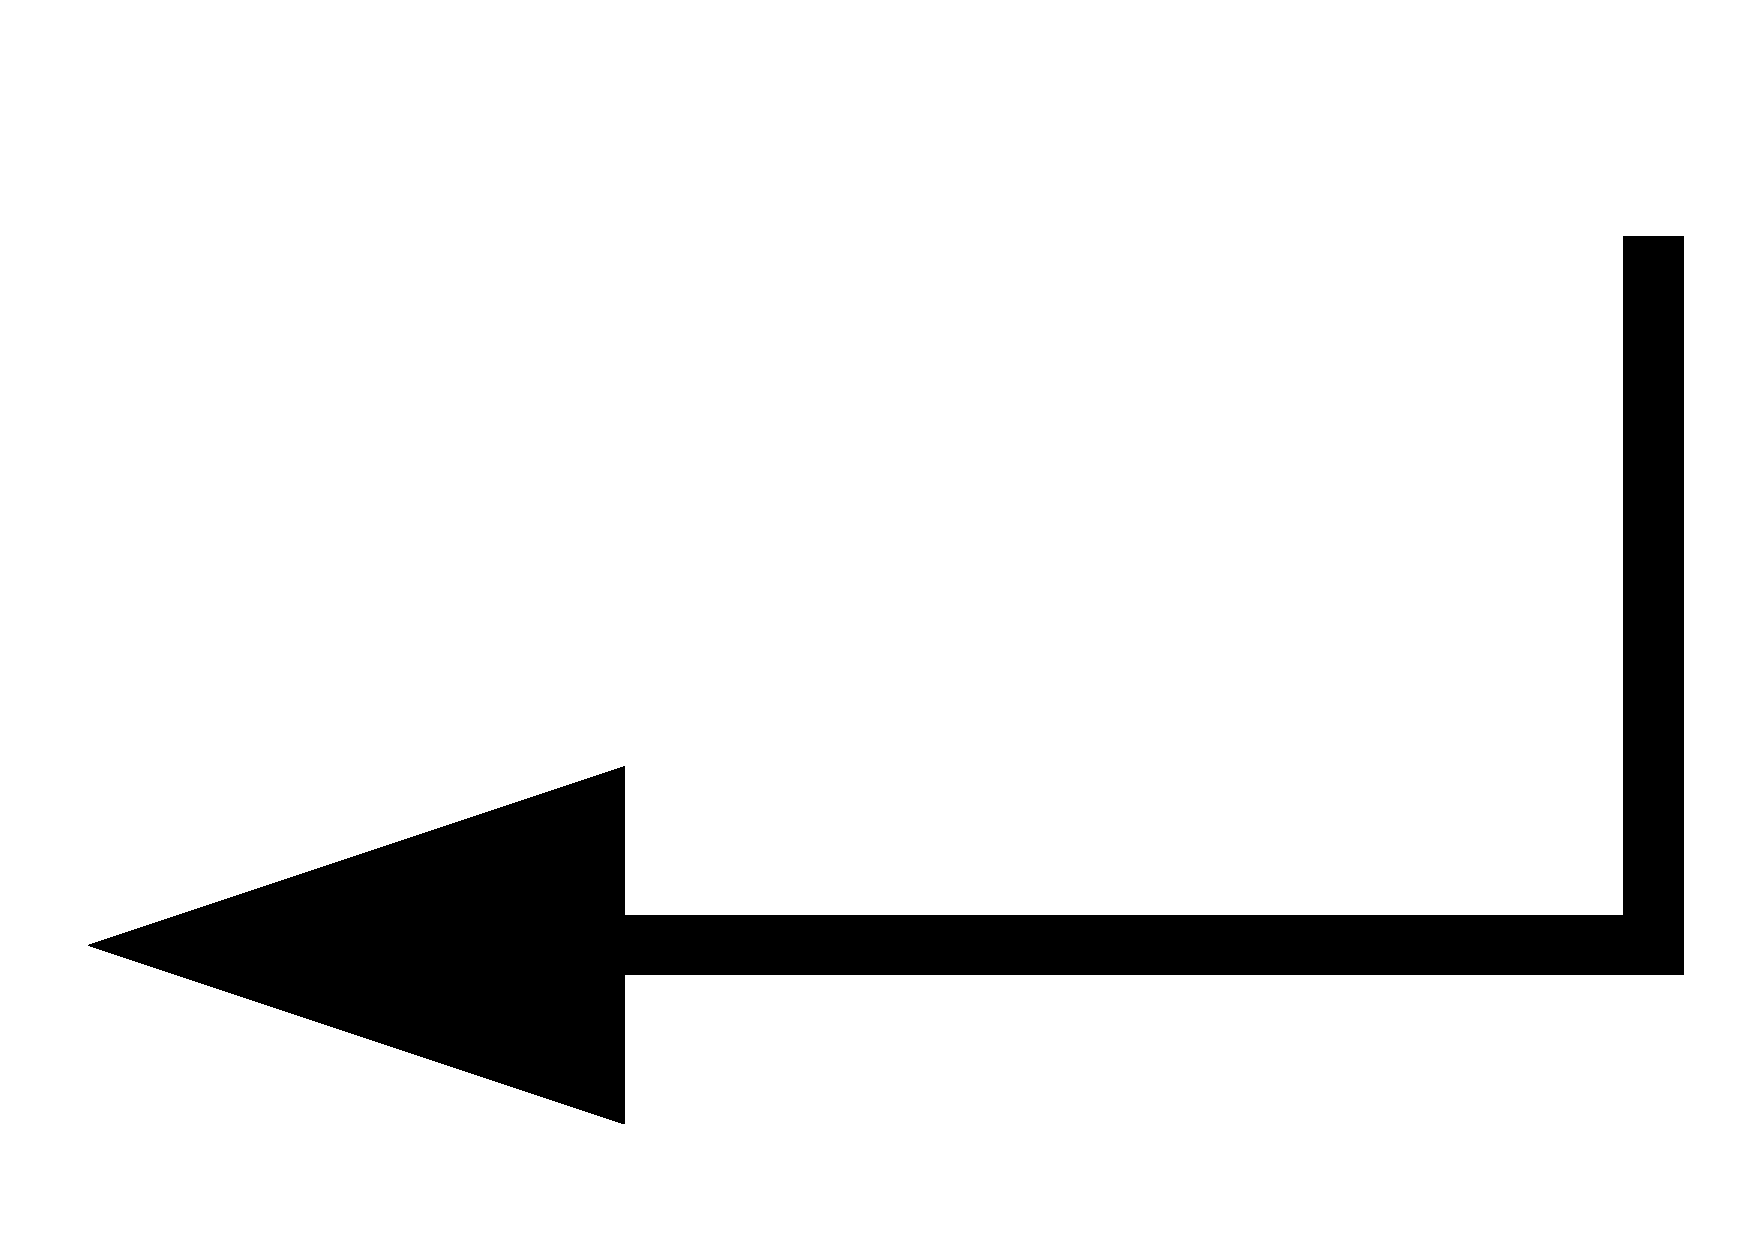
\includegraphics[width=1em]{figures/return-symbol}}}

%% Change how subfigures are labelled
\makeatletter
\renewcommand{\@thesubfigure}{\figurename~\thefigure\alph{subfigure}: }
\renewcommand{\thesubfigure}{\alph{subfigure}}
%%%\renewcommand{\p@subfigure}{\alph{subfigure}}
\makeatother

% No indents at start of paragraph, but paragraphs have blank lines
% between them
\setlength{\parindent}{0pt}
\setlength{\parskip}{2ex} 


%% \filename allows for _ but otherwise is formatted identically to
%% code. If using tildes (~) then use \mytilde command, inside
%% \texttt. Use the url package's command to define this, that way
%% hyperref doesn't see it as a hyperref!
\DeclareUrlCommand\filename{\urlstyle{tt}}
\newcommand{\email}[1]{\href{mailto:#1}{#1}}
\newcommand{\ccThreeUrl}{http://creativecommons.org/licenses/by-sa/3.0/}

%% Environment variables. Like \filename but prepends a $
\DeclareUrlCommand\envVar{\def\UrlLeft{\$}\urlstyle{tt}}
\DeclareUrlCommand\dosEnvVar{\def\UrlLeft{\%}\def\UrlRight{\%}\urlstyle{tt}}

\newcommand{\code}[1]{\texttt{#1}}

%% Use for menu selections etc
\newcommand{\myquote}[1]{\textcolor{MyQuoteColor}{\textsl{#1}}}

%% Define our own keypress command, based on keystroke
\newcommand{\keypress}[1]{\keystroke{#1}}

%% Units
%%\newcommand{\units}[2]{\mbox{\ensuremath{#1}\,#2}}
%%\newcommand{\dB}[1]{\mbox{\ensuremath{#1}\,dB}}
\newcommand{\dB}[1]{\SI{#1}{dB}}
\newcommand{\inch}[1]{\mbox{\ensuremath{#1}''}}
\newcommand{\kHz}[1]{\mbox{\ensuremath{#1}\,kHz}}
%\newcommand{\metre}[1]{\mbox{\ensuremath{#1}\,m}}
\newcommand{\km}[1]{\mbox{\ensuremath{#1}\,km}}
%% \newcommand{\MHz}[1]{\mbox{\ensuremath{#1}\,MHz}}
\newcommand{\MHz}[1]{\SI{#1}{\mega\hertz}}
\newcommand{\volt}[1]{\mbox{\ensuremath{#1}\,V}}
\newcommand{\bit}[1]{\mbox{\ensuremath{#1}\,bit}}

%%\newcommand{\degrees}[1]{\ensuremath{#1^\circ}}

\renewcommand{\textohm}{\ensuremath{\Omega}}
\newcommand{\kohm}[1]{\SI{#1}{\kilo\ohm}}


%%\newcommand{\pF}[1]{\units{#1}{pF}}
\newcommand{\pF}[1]{\SI{#1}{\pico\farad}}
\newcommand{\nF}[1]{\SI{#1}{\nano\farad}}
\newcommand{\uF}[1]{\SI{#1}{\micro\farad}}
%\newcommand{\nF}[1]{\units{#1}{nF}}
%\newcommand{\uF}[1]{\units{#1}{\ensuremath{\mu}F}}

%% Some simple abbreviations  
\newcommand{\ie}{i.e.}
\newcommand{\eg}{e.g.}
\newcommand{\etal}{\latin{et al.}}
\newcommand{\etc}{etc.}
%% Have warnings printed in light red box, with each item using a
%% STOP sign as a bullet
\newenvironment{warninglist}{%
  \begin{list}{\Stopsign}{}}{%
    \end{list}}
\newcommand{\warningbox}[1]{\noindent
  \colorbox{MyLightRed}{\parbox[l]{\textwidth}{%
      \begin{warninglist}\item #1\end{warninglist}}} \newline}

%% Have help information printed in light blue box, with each item using an
%% information sign as a bullet
\newenvironment{helplist}{%
  \begin{list}{\Info}{}}{%
    \end{list}}
\newcommand{\helpbox}[1]{\noindent
  \colorbox{MyLightBlue}{\parbox[l]{\textwidth}{%
      \begin{helplist}\item #1\end{helplist}}} \newline}

%% Verbatim-like environment for code.
\DefineVerbatimEnvironment{Code}{Verbatim}%
{frame=single,commandchars=\\\{\}}
\DefineVerbatimEnvironment{Cmd}{Verbatim}%
{frame=single,label=\linuxLogo,framesep=5mm,commandchars=\\\{\}}
\DefineVerbatimEnvironment{LinuxCmd}{Verbatim}%
{frame=single,label=\linuxLogo,framesep=5mm,commandchars=\\\{\}}
\DefineVerbatimEnvironment{WindowsCmd}{Verbatim}%
{frame=single,label=\windowsLogo,framesep=5mm,commandchars=\\\{\}}

%% \DefineVerbatimEnvironment{Cmd}{LinuxCmd}{}


\newcommand{\todo}[1][]{\fcolorbox{magenta}{MyLightMagenta}{\mbox{\textcolor{black}{TO DO\ifthenelse{\equal{#1}{}}{}{: #1}}}}}

\newcommand{\figscale}{1.0}

%% Have subsubsections numbered
\setcounter{secnumdepth}{5}
\setcounter{tocdepth}{5}

\begin{document}

\title{AuroraWatchNet magnetometer manual}
\author{Steve Marple, \\
Lancaster University.}
\date{\today}
\maketitle
\thispagestyle{empty}
\frontmatter
\pagestyle{headings}

\clearpage  
\phantomsection  
% \thispagestyle{empty}
\chapter{Licence}
This document is made available under the \href{\ccThreeUrl}{Creative
  Commons Attribution-ShareAlike 3.0 Unported Licence}.

\begin{center}
\href{\ccThreeUrl}{
\includegraphics{images/by-sa}}
\end{center}

\clearpage  
\phantomsection  
\addcontentsline{toc}{chapter}{\contentsname}  
\tableofcontents

\newpage
\phantomsection  
\addcontentsline{toc}{chapter}{\listfigurename}  
\listoffigures

%% -----------------------------
\newpage
\phantomsection  
\addcontentsline{toc}{chapter}{\listtablename}  
\listoftables


%% List of abbreviations. Include all useful ones. Those which are not
%% used are not included in the table.

\abbrev{\adc}{ADC}{analogue to digital converter}
\abbrev{\api}{API}{application programming interface}
\abbrev{\bgs}{BGS}{Bitish Geological Survey}
\abbrev{\cpu}{CPU}{central processing unit}
\abbrev{\dhcp}{DHCP}{dynamic host configuration protocol}
\abbrev{\dip}{DIP}{dual-inline package}
\abbrev{\dns}{DNS}{domain name system}
\abbrev{\dtr}{DTR}{data terminal ready}
\abbrev{\eeprom}{EEPROM}{electrically erasable programmable read-only memory}
\abbrev{\esd}{ESD}{electro-static discharge}
\abbrev{\fat}{FAT}{file allocation table}
\abbrev{\fet}{FET}{field-effect transistor}
\abbrev{\gpu}{GPU}{graphics processing unit}
\abbrev{\gui}{GUI}{graphical user interface}
\abbrev{\hmac}{HMAC}{hash-based message authentication code}
\abbrev{\http}{HTTP}{hypertext transfer protocol}
\abbrev{\https}{HTTPS}{hypertext transfer protocol secure}
\abbrev{\ic}{IC}{integrated circuit}
\abbrev{\itwoc}{I2C}{inter-integrated circuit (bus)}
\abbrev{\ir}{IR}{infra-red}
\abbrev{\ism}{ISM}{Industrical, scientific and medical (radio band)}
\abbrev{\isp}{ISP}{in-circuit serial programmer (sometimes abbreviated as ICSP)}
\abbrev{\ip}{IP}{internet protocol}
\abbrev{\jtag}{JTAG}{joint test action group}
\abbrev{\led}{LED}{light emitting diode}
\abbrev{\mdfive}{MD5}{message digest 5}
\abbrev{\nfs}{NFS}{network file system}
\abbrev{\ntp}{NTP}{network time protocol}
\abbrev{\ota}{OTA}{over the air (as in firmware updates)}
\abbrev{\pcb}{PCB}{printed circuit board}
\abbrev{\PoE}{PoE}{power over ethernet}
\abbrev{\psu}{PSU}{power supply unit}
\abbrev{\rfi}{RFI}{radio-frequency interference}
\abbrev{\rtc}{RTC}{real-time clock}
\abbrev{\samnet}{SAMNET}{Sub-Auroral Magnetometer Network}
\abbrev{\sd}{SD}{secure digital}
\abbrev{\ssh}{SSH}{secure shell}
\abbrev{\soic}{SOIC}{small outline integrated circuit}
\abbrev{\tcp}{TCP}{transmission control protocol}
\abbrev{\ttl}{TTL}{transistor-transistor logic}
%% \url is already a command, use \URL for the abbreviation
\abbrev{\URL}{URL}{uniform resource locator}
\abbrev{\usb}{USB}{universal serial bus}
\abbrev{\ut}{UT}{universal time}
\abbrev{\utc}{UTC}{coordinated universal time}
\abbrev{\udp}{UDP}{user datagram protocol}


\mainmatter
%% Allow for sloppy wordbreaking to avoid text spilling into the
%% margin (eg as a result of \filename and other non-breaking text)
\sloppy
\part{Introduction}
\chapter{Overview of the hardware}

\section{Introduction}
The magnetometer is designed for low-power operation, simple
installation and ease of construction. The entire design is open
source, allowing anyone with reasonable soldering ability to construct
one.

The magnetometer has two major parts, the base unit and the sensor
unit (\figurename~\ref{fig:system-overview}). The sensor unit is located
outdoors, away from buildings, cars and other sources of human
disturbance. It is battery powered and communicates with the base unit
by a radio link (\MHz{433} or \MHz{868}), enabling the sensor to be
installed without any wiring to the base unit. The base unit is placed
indoors and should be positioned such that there are the minimum
number of walls between it and the sensor unit.

\begin{figure}
  \centering
  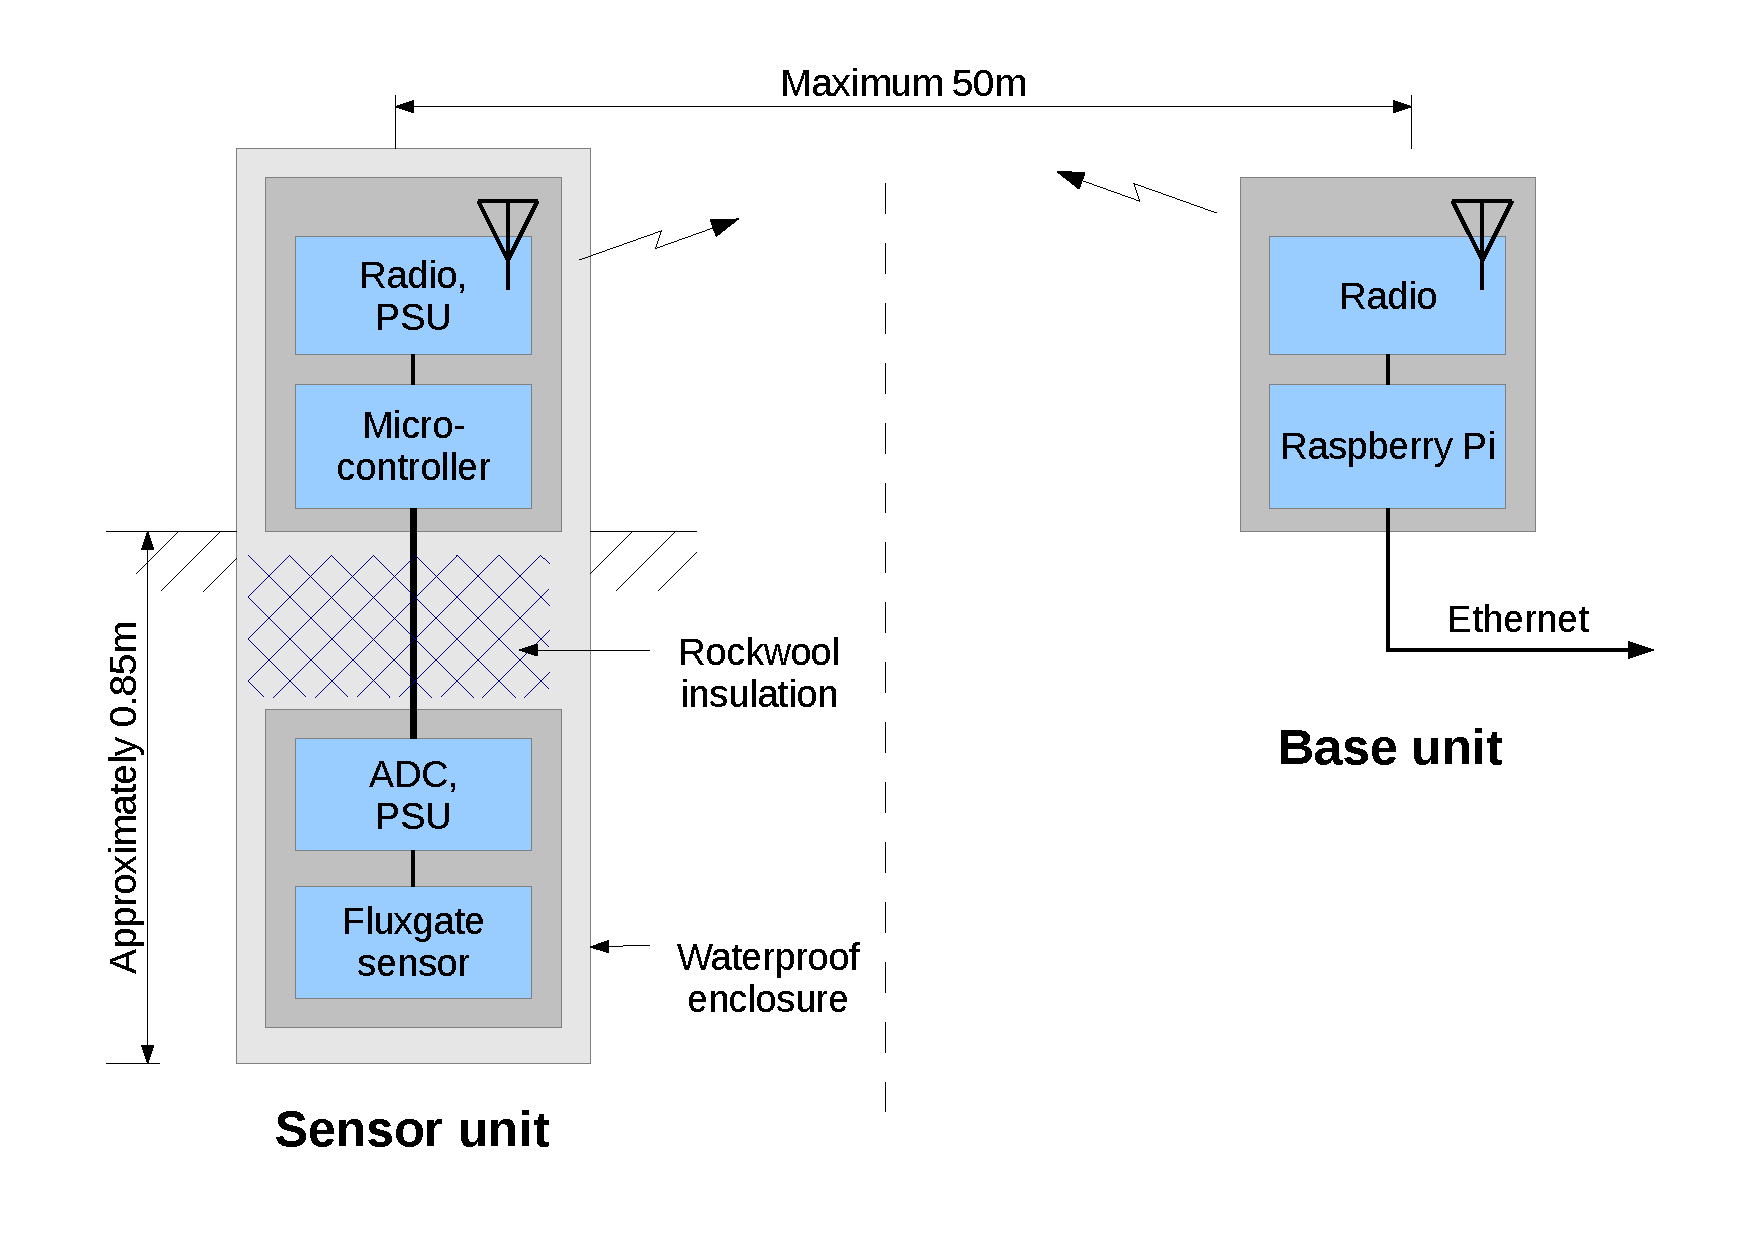
\includegraphics[keepaspectratio,width=\textwidth]{%
    calunium-mag/images/system-overview}
  \caption[System overview]%
  {System overview.}
  \label{fig:system-overview}
\end{figure}

\section{Sensor unit}

The sensor unit (figure~\ref{fig:sensor-unit}) is contained inside a
waterproof enclosure approximately \SI{1.1}{\metre} high which is
partially buried to reduce temperature variations and to provide a
stable foundation. The sensor itself is placed at the bottom of the
enclosure, approximately \SI{0.85}{\metre} below ground. The
microcontroller, radio module and battery are positioned in the top
part of the enclosure, above ground level. Insulating material (\eg\
rockwool) is used to fill the space in-between.

The
\href{http://blog.stevemarple.co.uk/search/label/Calunium}{Calunium}
microcontroller board is based on the popular
\href{http://arduino.cc}{Arduino} platform but uses the more powerful
Atmel ATmega1284P microcontroller.

\begin{figure}[!h]
  \centering
  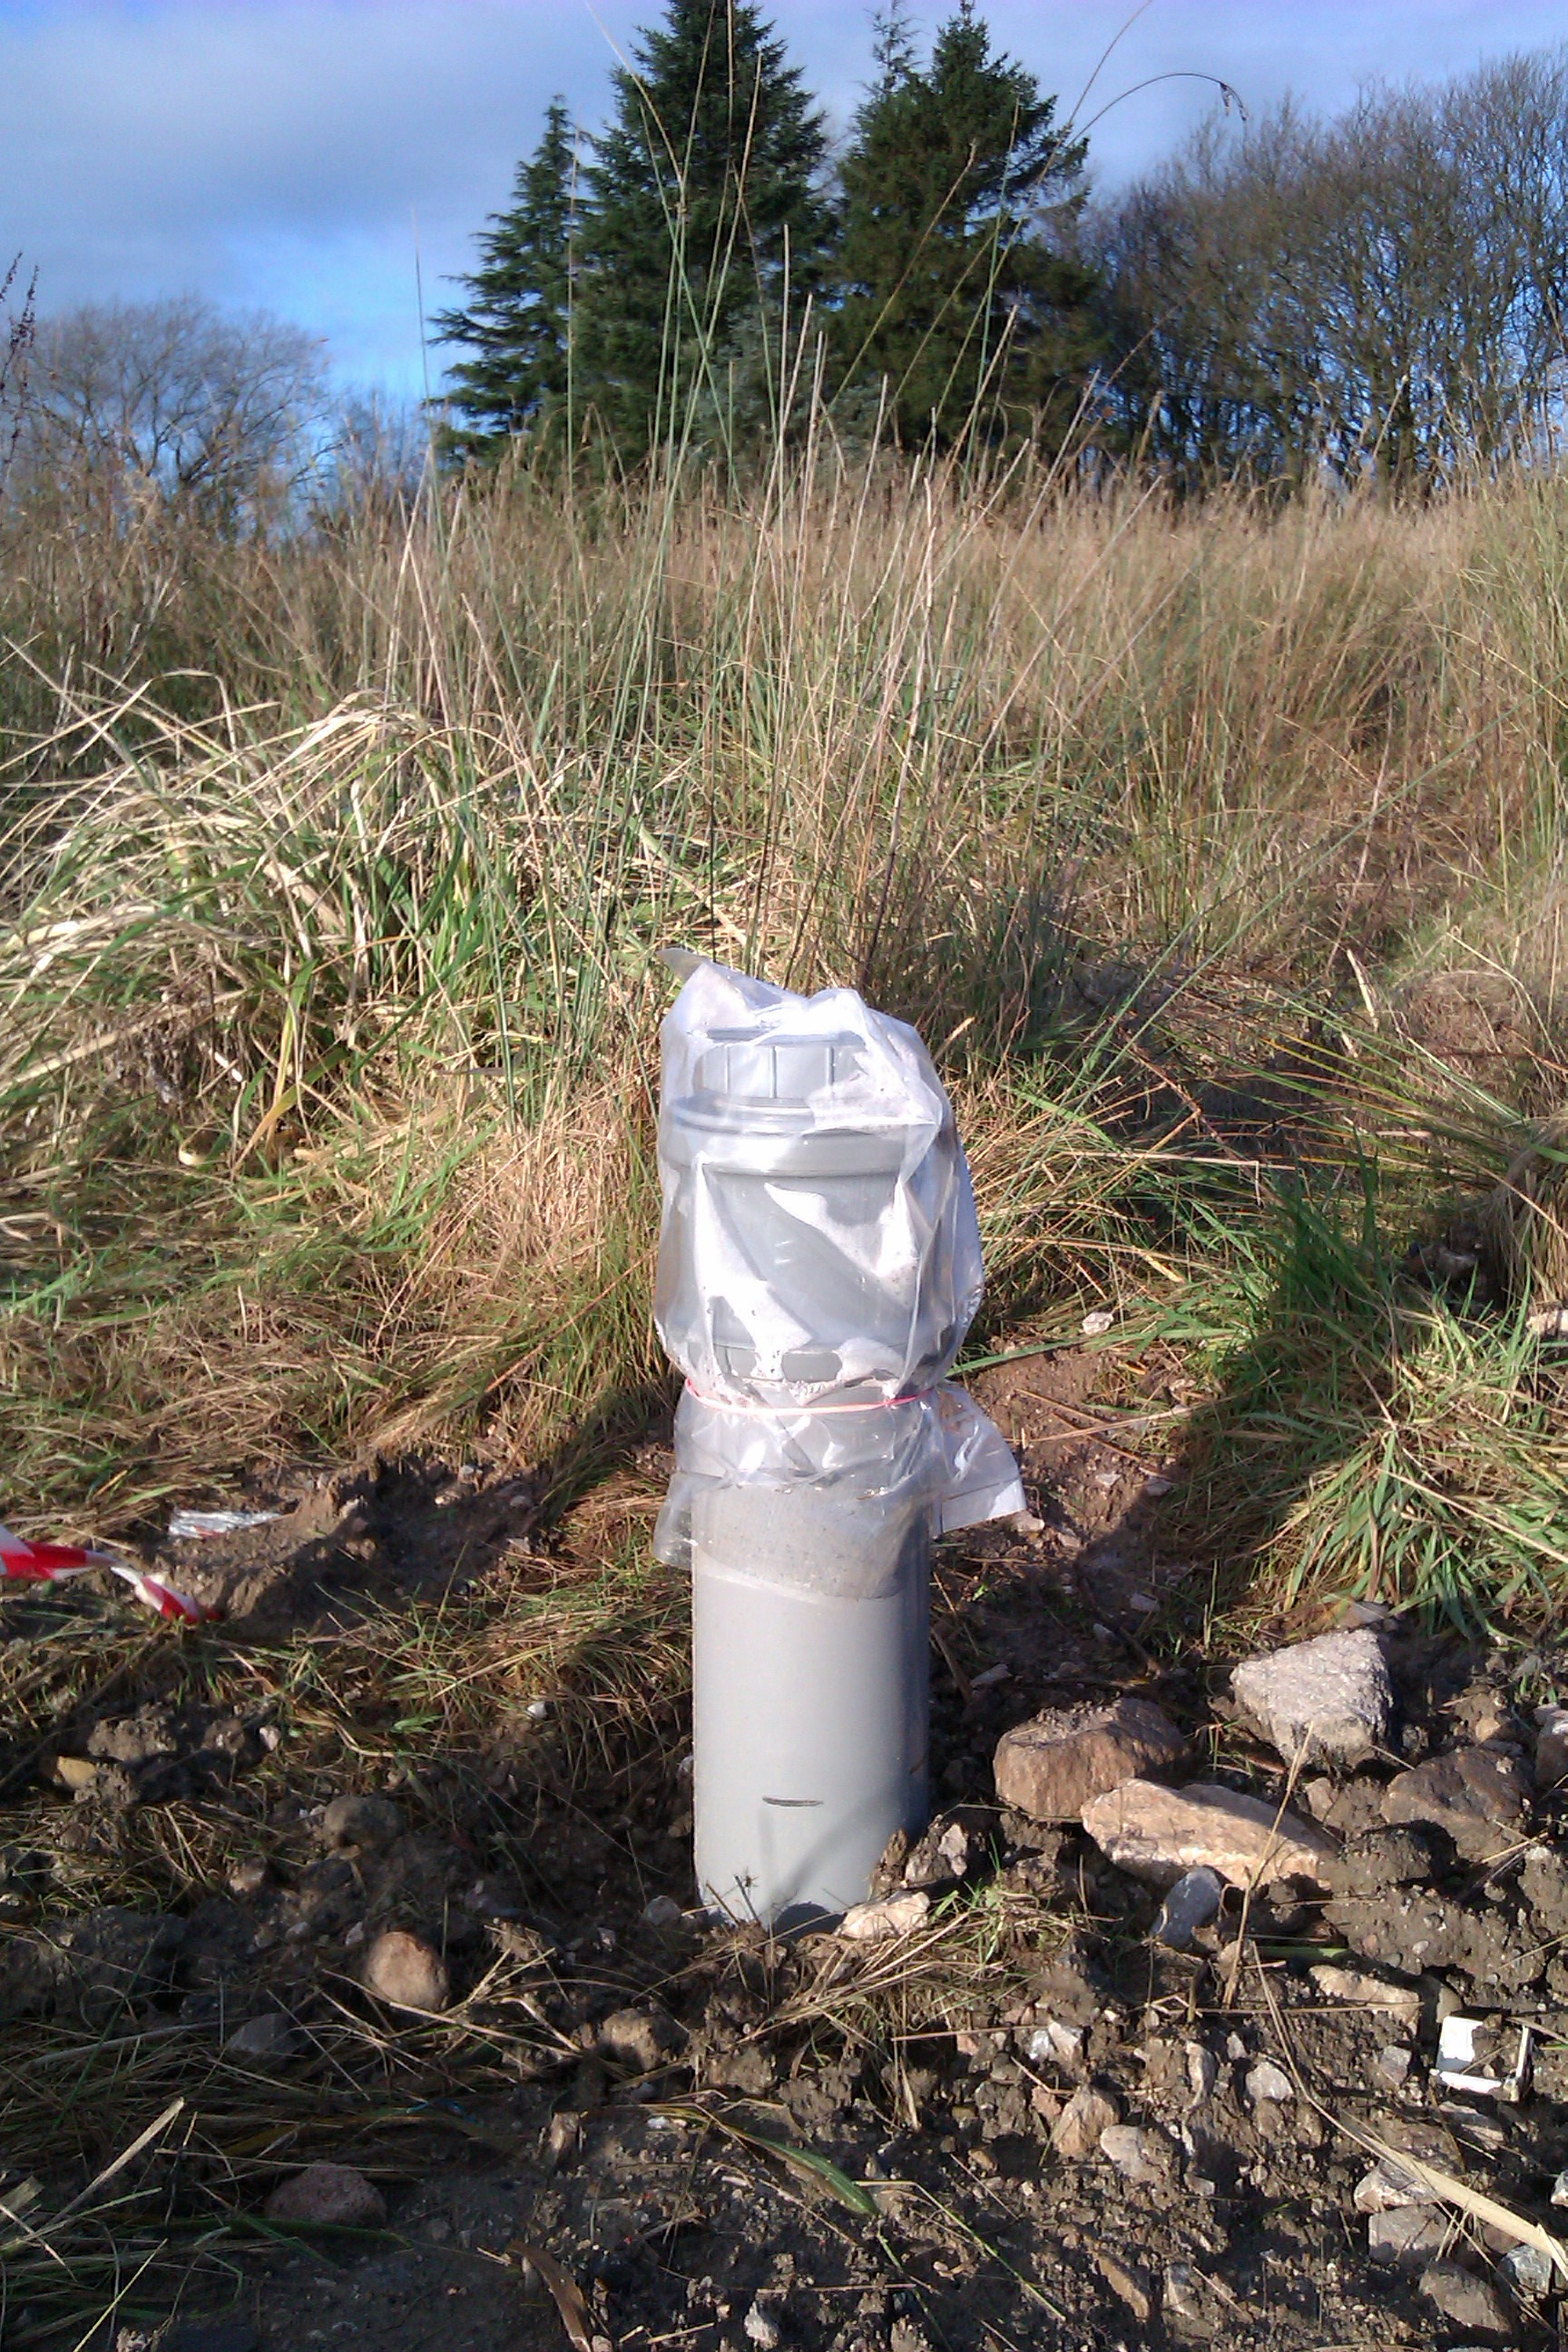
\includegraphics[keepaspectratio,height=10cm]{images/sensor-unit}
  \caption[Sensor unit]{%
    Sensor unit. \photoCredit{Steve Marple}{\ccBySaTwo}{%
      http://www.flickr.com/photos/stevemarple/8499204572/} 
  }
  \label{fig:sensor-unit}
\end{figure}

\begin{figure}
  \centering
  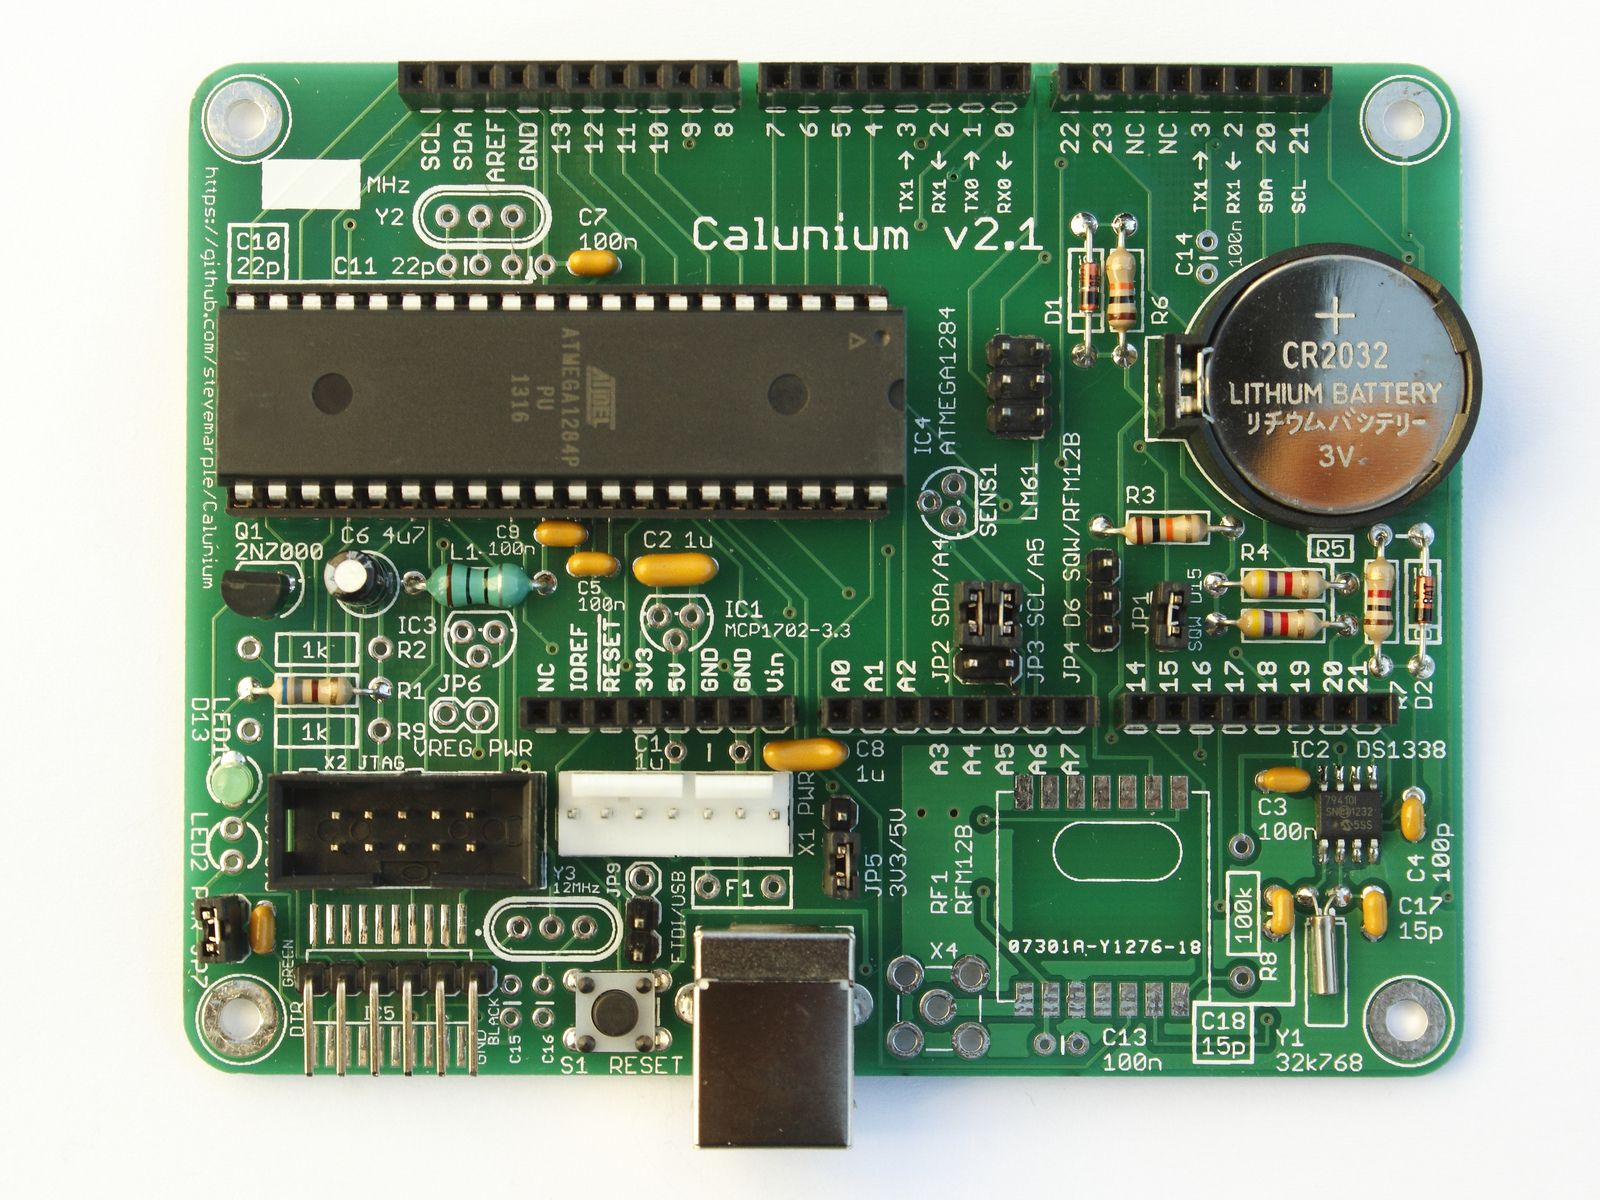
\includegraphics[keepaspectratio,width=\textwidth]{%
    images/calunium-v2-1}
  \caption[Calunium microcontroller PCB]{%
    Calunium microcontroller \pcb. %
    \photoCredit{Steve Marple}{\ccBySaTwo}{%
      http://www.flickr.com/photos/stevemarple/10786865096/}}
  \label{fig:calunium}
\end{figure}

\begin{figure}
  \centering
  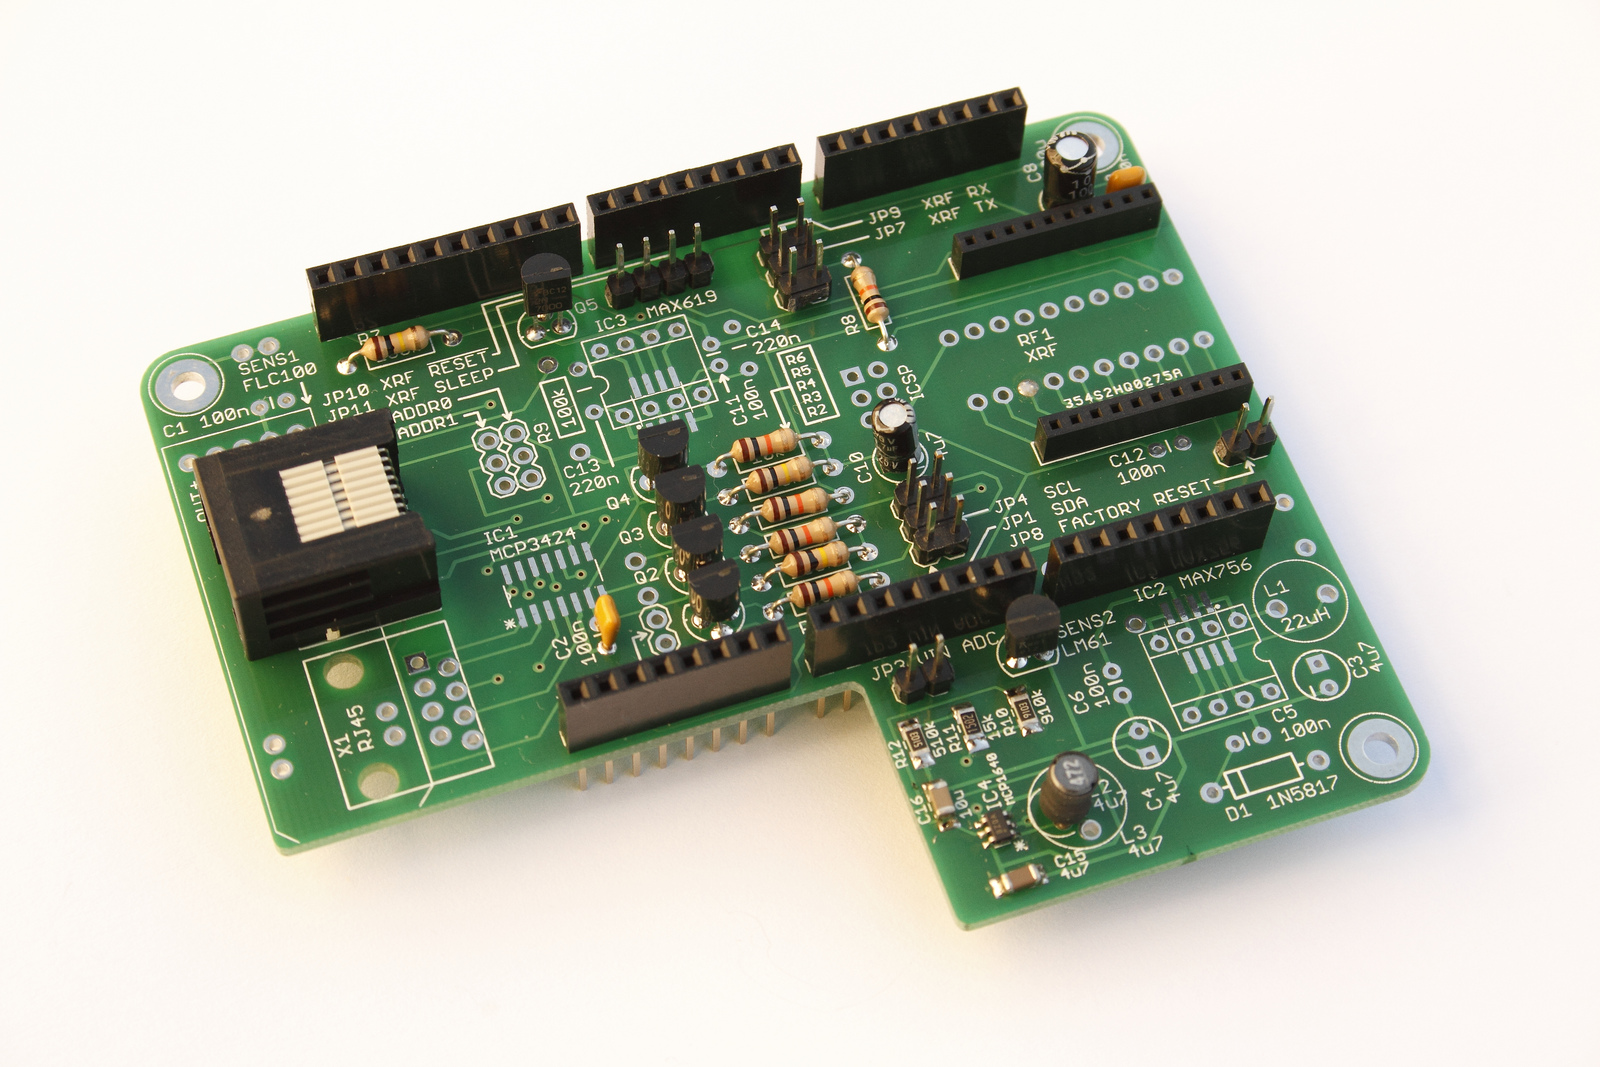
\includegraphics[keepaspectratio,width=\textwidth]{%
    images/flc100-shield}
  \caption[FLC100 shield]{The FLC100 shield fits onto the Calunium
    microcontroller \pcb. \photoCredit{Steve Marple}{\ccBySaTwo}{%
      http://www.flickr.com/photos/stevemarple/10787109594/}}
  \label{fig:flc-100-shield}
\end{figure}

\begin{figure}
  \centering
  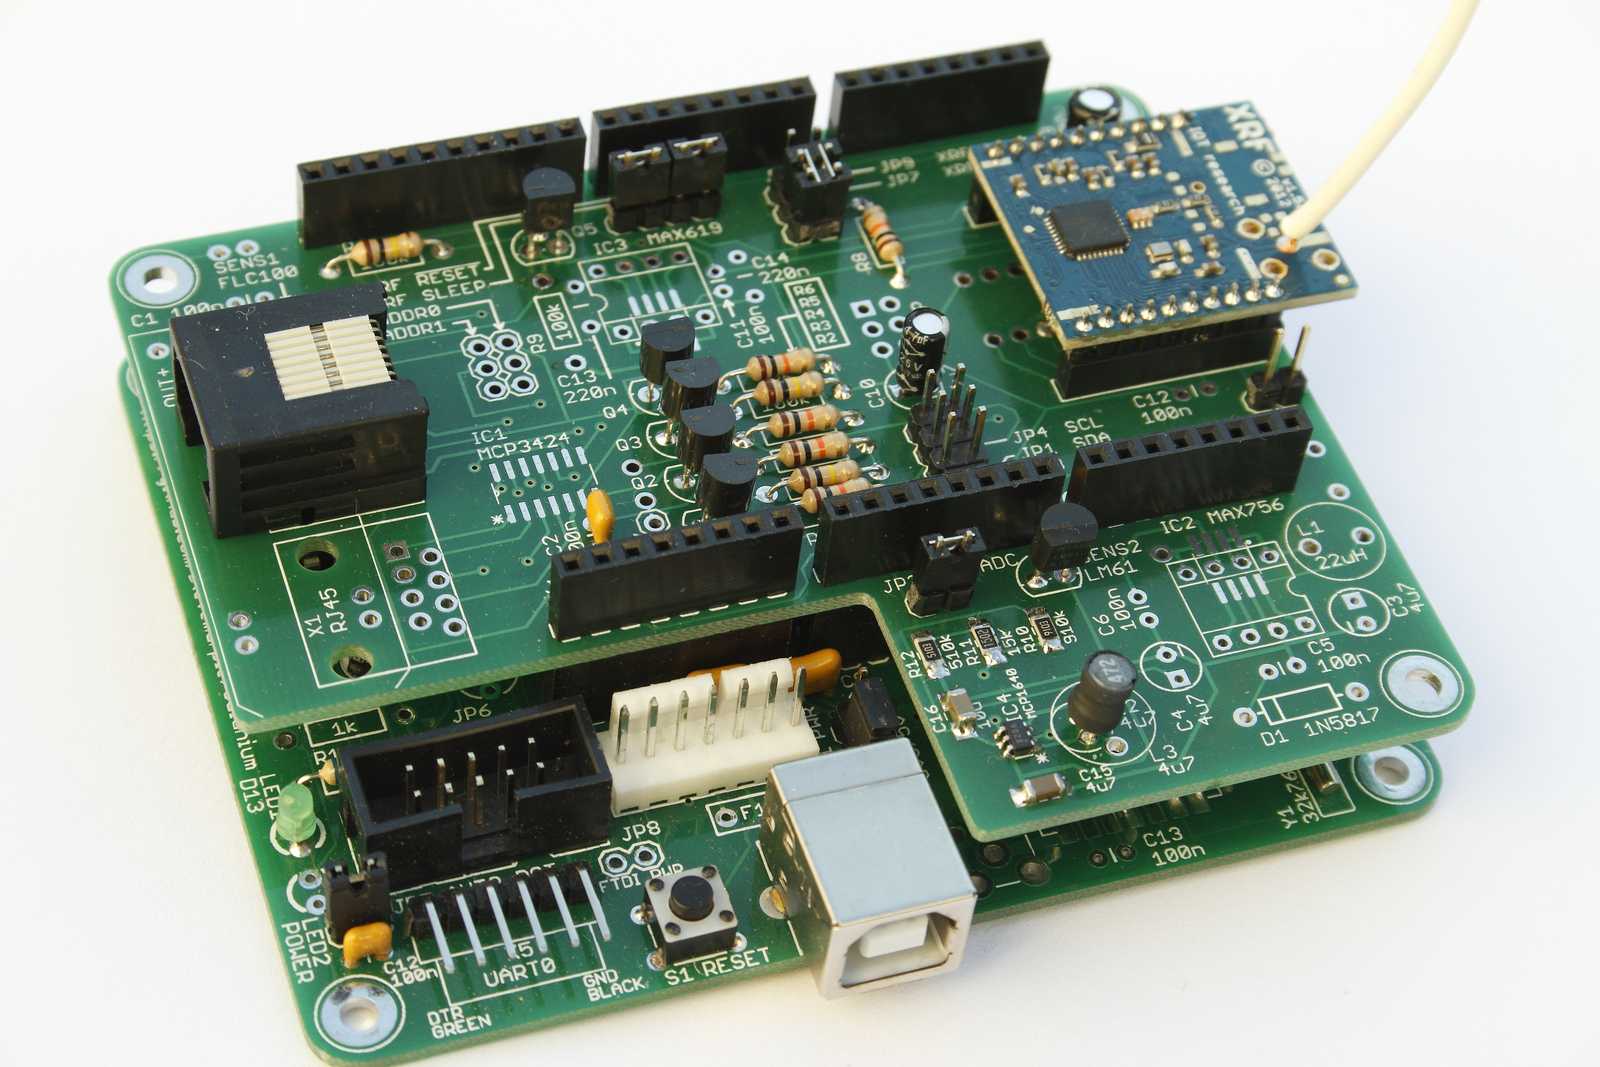
\includegraphics[keepaspectratio,width=\textwidth]{%
    images/calunium-flc100-shield.jpg}
  \caption[Calunium microcontroller board and FCL100 shield]{%
    Calunium microcontroller board and FCL100 shield. 
    \photoCredit{Steve Marple}{\ccBySaTwo}{%
      http://www.flickr.com/photos/stevemarple/10913562526/}}
  \label{fig:calunium-flc-100-shield}
\end{figure}

\clearpage
\section{Base unit}

The base unit is a \href{http://www.raspberrypi.org/‎}{Raspberry Pi}
single-board computer with a radio transceiver unit. The Ethernet
interface of the Raspberry Pi is used to send the magnetic field
measurements to AuroraWatch UK. When the Raspberry Pi is accessed over
the network with Secure Shell (\ssh) a display and keyboard are not
needed. The Raspberry Pi runs the Raspbian linux distribution. The
receiving software is written in Python.

\begin{figure}[!h]
  \centering
  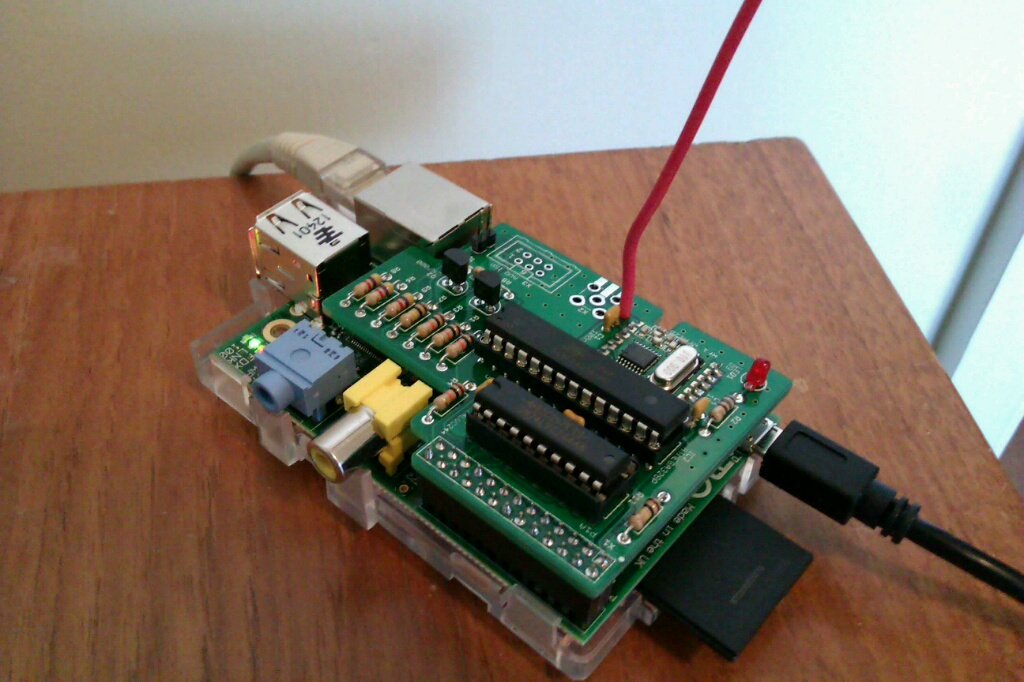
\includegraphics[keepaspectratio,height=10cm]{images/base-unit}
  \caption[Base unit]{%
    Base unit. \photoCredit{Steve Marple}{\ccBySaTwo}{%
      http://www.flickr.com/photos/stevemarple/10787215844/}}
  \label{fig:base-unit}
\end{figure}


\part{Construction}
\chapter{Beginning construction}

\section{Anti-static precautions}

\section{Tools required}

\begin{itemize}
\item Soldering iron.
\item Sidecutters.
\item Small pliers.
\item In-circuit serial programmer for Atmel AVR microcontrollers,
  \eg, \href{http://www.atmel.com/tools/AVRDRAGON.aspx}{Atmel AVR Dragon}.
\item \usb\ to \ttl\ serial converter for \volt{3.3} operation, \eg, FTDI
  TTL-232R-3V3.
\item Digital multimeter.
\item Solderless breadboard (optional).
\end{itemize}

\section{Order of assembly}

For ease of access components should normally be fitted in order of
increasing size, particularly increasing height. If this order is not
observed it can ver very difficult to access the pads of surface mount
devies. It is also preferable that \emph{passive} components
(resistors, capacitors, inductors and crystals) are fitted before
semiconductors (field-effect transistors, integreated circuits). This
is because the semiconductors are easily damaged by electro-static
discharge (sometimes this damage isn't immediately obvious). It is
therefore more convenient to fit as many components as possible before
fitting the semiconductors, at which point \esd\ precautions should be
followed. As field-effect transistors are particularly vulnerable to
damage by \esd\ it is recommended they are fitted as late as possible.
From these guidelines the following order is recommended.
\begin{itemize}
\item Surface-mount passive components.
\item Surface-mount semiconductors.
\item Through-hole passive components.
\item Through-hole semiconductors (\fet s last).
\item Switches.
\item Connectors, battery holders.
\end{itemize}

The first \pcb\ to be assembled is the FLC100 shield, this board
provides the power to the system and will enable you to test each part
correctly.

\chapter{Calunium assembly}

\section{Introduction}

The Calunium microcontroller development board is intended to be a
flexible system for both development and embedded use. As such it has
various hardware options and careful attention must be paid to
assembling it for optimum performance. Parts which are not needed are
omitted to lower power consumption (\eg, power LED, USB controller).

\section{Calunium version 2.0 and version 2.1}

\begin{figure}
  \centering
  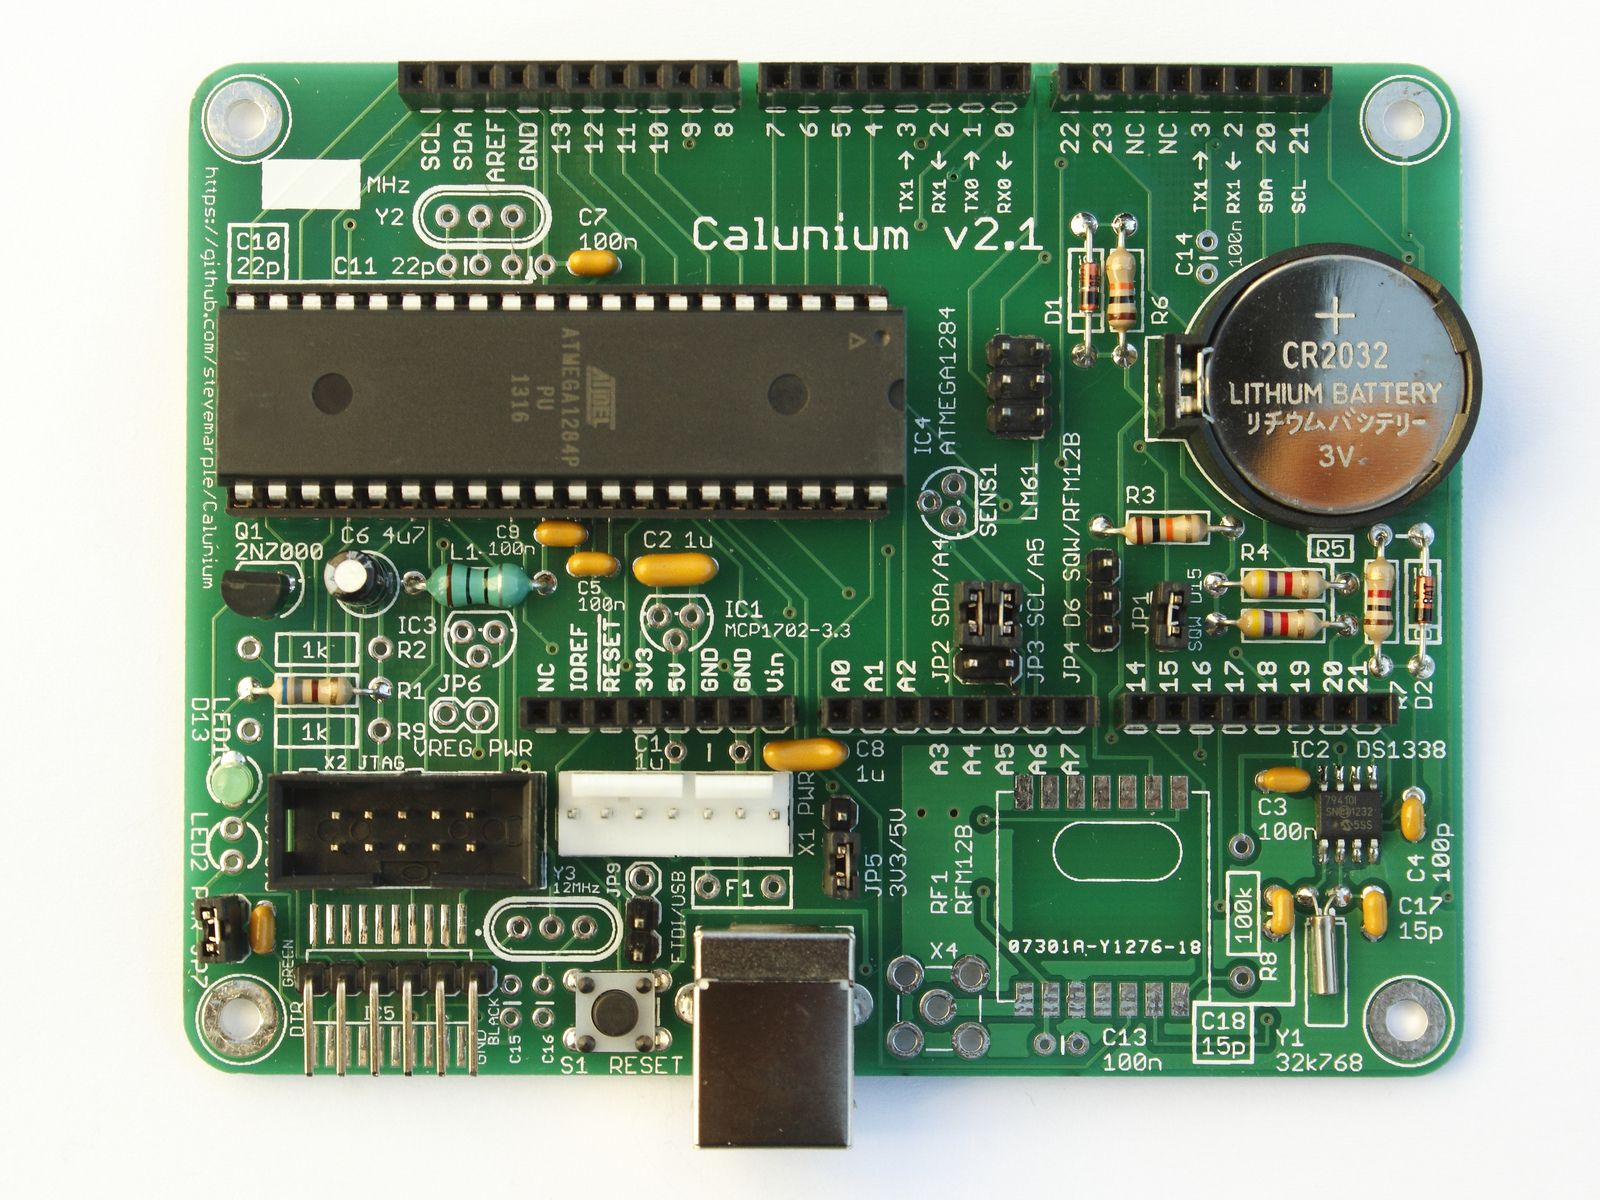
\includegraphics[keepaspectratio,width=\textwidth]{%
    images/calunium-v2-1}
  \caption[Completed Calunium v2.1]{%
    Completed Calunium v2.1. \photoCredit{Steve Marple}{\ccBySaTwo}{%
      http://www.flickr.com/photos/stevemarple/10786865096/}}
  \label{fig:calunium-version-2.1}
\end{figure}

\subsection{Order of assembly}

Fit components in order:
\begin{buildorder}
\item IC2. The standard real-time clock is the MicroChip MCP90410 but
  MicroChip MCP79411 or MCP79412 can be used without any other
  changes.
  It is also possible to fit the Maxim DS1338-33 real-time clock,
  but see below for changes.
\item Y1 (\kHz{32.768}).
\item R1, fit a \ohm{680} resistor. Ignore the \kohm{1} marking; a
  lower value resistor is used to enable the green LED to be seen
  more clearly in daylight.
\item R7 (\kohm{1}). Do not fit if using the DS1338-33 real-time
  clock. Instead link between R7 and D2 at the end nearest the \rtc\
  battery, as indicated by the white line on the silkscreen. The wire
  will bypass both R7 and D2 which are not required for the DS1338-33.
\item R4, R5 (\kohm{4.7}).
\item R3, R6 (\kohm{10}).
\item L1 (\uH{10}).
\item 40~pin socket for IC4.
\item C4 (\pF{100}).
\item C3, C5, C7, C9, C12 (\nF{100}).
\item C2, C8 (\uF{1}).
\item D1, D2 (BAT85). Do not fit D2 if using the DS1338-33 real-time clock.
\item LED1 (green LED). The cathode is nearest LED2, see
  figure~\ref{fig:calunium-led-orientation}.
\item C6 (\uF{4.7}).
\item ICSP header ($2 \times 3$ jumper block). See
  \figurename~\ref{fig:icsp-header}.
\item JP2 and JP3. Fit as combined $2 \times 3$ jumper block.
\item JP1, JP7 ($1 \times 2$ jumper).
\item JP4, JP5 ($1 \times 5$ jumper).
\item X5 ($1 \times 6$ right-angle or vertical header for UART0).
\item S1 (reset switch).
\item Arduino headers. \todo[Add description]
\item C17, C18 (\pF{15}). Do not fit if using DS1338-33 \rtc. For
  Calunium version 2.0 the capacitors must be fitted on the reverse
  side of the board (see \figurename~\ref{fig:calunium-rtc-caps-hack}
  as no specific mounting holes exist (error caused by using an
  earlier, incorrect datasheet which did not show the load
  capacitors).
\item X1 (Molex power header). Ensure correct orientation, with the
  backplate closest to the Arduino headers.
\item \todo[Add component name] (\rtc\ battery holder).
\item Q1 (2N7000). This item is very sensitive to damage by
  electrostatic discharge!
\item Battery (CR2032). Check that the battery backup pin (3) on the
  \rtc\ measures \volt{3.0}.
\item \todo[Fit shunts to jumpers \ldots]
\end{buildorder}
Do not fit the ATmega1284P microcontroller until after testing the
board power supplies.

\begin{figure}
  \centering
  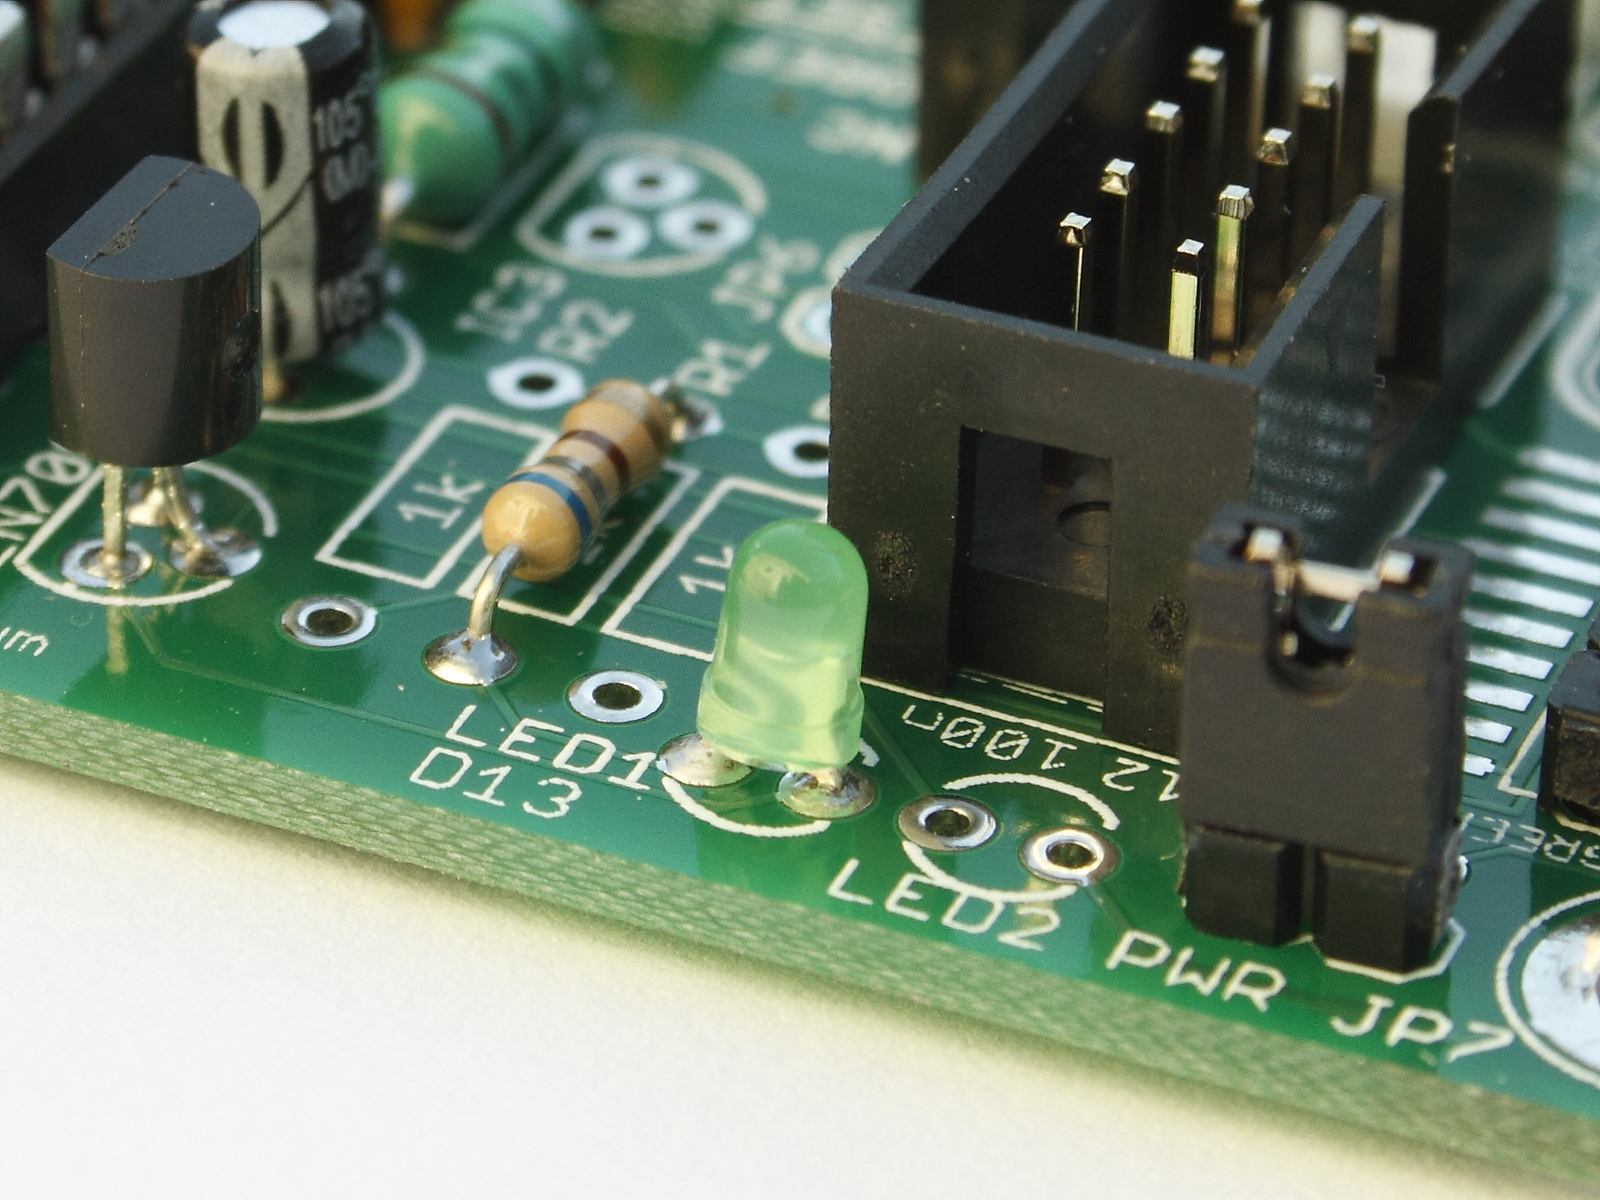
\includegraphics[keepaspectratio,width=10cm]{%
    images/calunium-led-orientation}
  \caption[LED orientation]{\led\ orientation. \photoCredit{%
      Steve Marple}{\ccBySaTwo}{%
      http://www.flickr.com/photos/stevemarple/10786846715/}}
  \label{fig:led-orientation}
\end{figure}
\begin{figure}
  \centering
  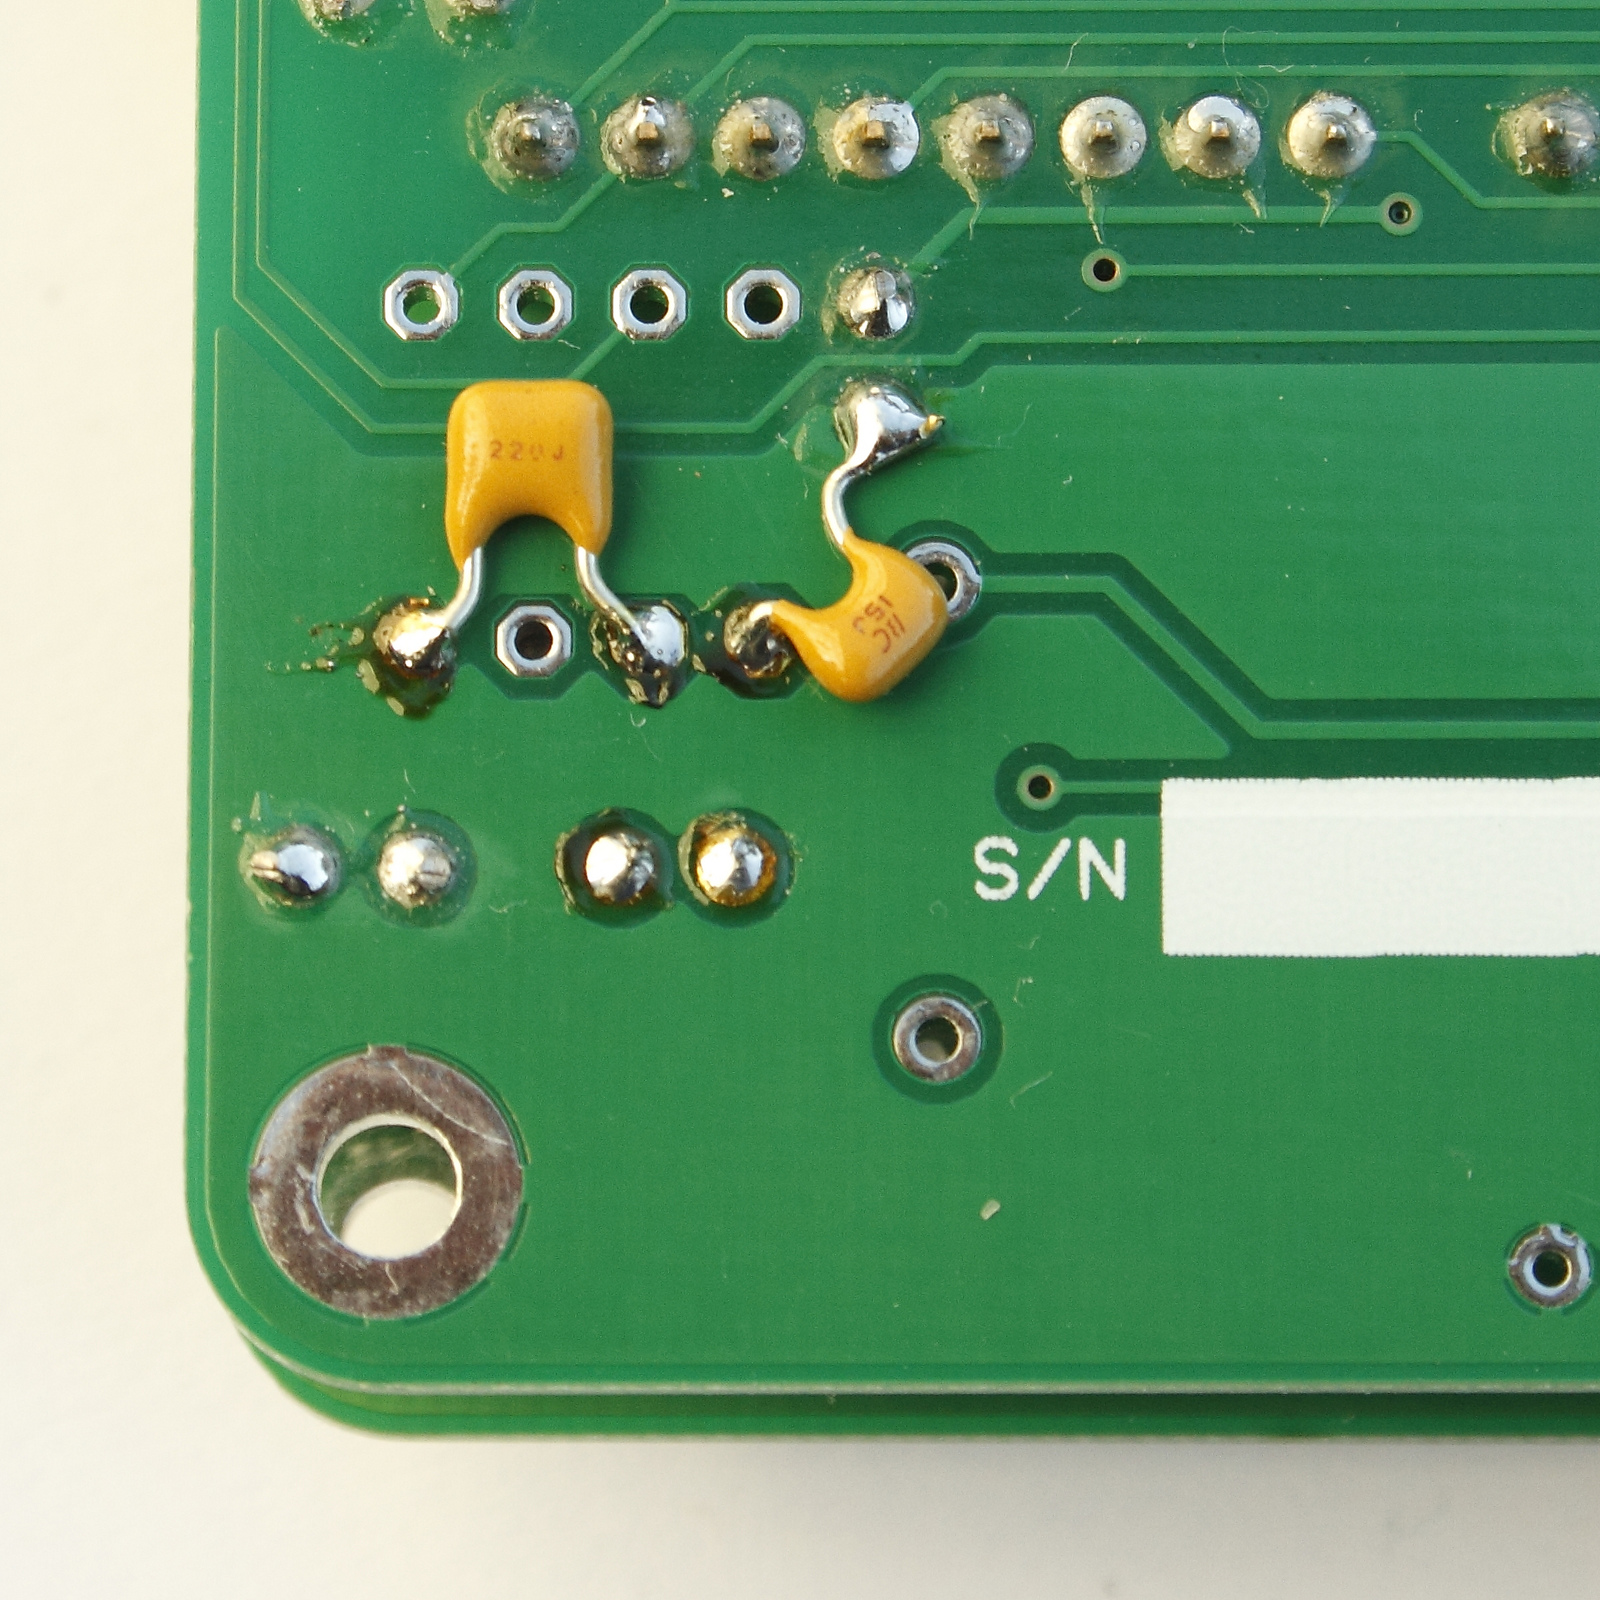
\includegraphics[keepaspectratio,width=10cm]{%
    images/calunium-rtc-caps-hack}
  \caption[Real-time clock load capacitors (Calunium v~2.0)]{%
    Real-time clock load capacitors (Calunium v~2.0). \photoCredit{%
      Steve Marple}{\ccBySaTwo}{%
      http://www.flickr.com/photos/stevemarple/10787041263/}}
  \label{fig:calunium-rtc-caps-hack}
\end{figure}


\begin{landscape}
  \begin{figure}[p]
    \centering
    \includegraphics[keepaspectratio,width=28cm,height=16cm]{%
      ../../hardware/Calunium/hardware/pcb/Calunium_v2/Calunium_v2_sch}  
    \caption{Calunium v.~2.0 circuit diagram.}
    \label{fig:calunium-v2.0-cct-diag}
  \end{figure}
  \begin{figure}[p]
    \centering
    % Use symbolic link for image to avoid a filename with a dot in
    % the main part of the name. This enables the extension to be left
    % off for easy processing with either latex or pdflatex.
    \includegraphics[keepaspectratio,width=28cm,height=16cm]{%
      images/Calunium_v2_1_sch}
    \caption{Calunium v.~2.1 circuit diagram.}
    \label{fig:calunium-v2.1-cct-diag}
  \end{figure}
\end{landscape}

\section{Testing the board}

\section{Programming the firmware}

These instructions assume you are using the Atmel AVR Dragon in \isp\
mode but adapting them to suit your programmer should be
straightforward; see the \filename{avrdude} manual page for further
information.

\subsection{Programming the bootloader}

Power up the Calunium board and connect the programmer. Ensure the
cable is correctly orientated at both ends. The bootloader can be
compiled and programmed simply, as user \piUser: \todo[Check directory]
\begin{Cmd}
  cd /home/pi/xboot
  make clean
  make SHELL=bash calunium_8MHz_RC_ISP.conf.mk program
\end{Cmd}
\todo: ignore lock bit verification errors.

If the bootloader is correctly programmed the green \led\ connected to
D13 on the Calunium \pcb\ should flash at about \Hz{1}.

\subsection{Programming the magnetometer firmware}
Ensure that the shunt marked ``AUTO RST'' is fitted, and that the
shunt marked ``FTDI PWR'' is omitted. Connect the FTDI cable and
identify the USB device file; as user \piUser:
\begin{Cmd}
  dmesg | tail
\end{Cmd}

Look for a line containing text similar to
\begin{Cmd}
  FTDI USB Serial Device converter now attached to ttyUSB0
\end{Cmd}
For the case above the device file \filename{/dev/ttyUSB0}. Now
program the microcontroller using the xboot bootloader. Replace
\filename{/dev/ttyUSB0} with the device file one your system. As user
\piUser:
\begin{Cmd}
  cd /home/pi/AuroraWatchNet/firmware/magnetometer
  avrdude -p atmega1284p -b 38400 -c avr109 -P /dev/ttyUSB0 \textbackslash
      -U flash:w:xrf_rf12-0.10a.bin:r
\end{Cmd}


\helpbox{Whilst it is possible to program the firmware using the AVR
  Dragon alone this approach ensures that the xboot bootloader is
  present and functions correctly, allowing the microcontroller
  firmware to be updated over the radio link.}

\chapter{Calunium firmware}

\chapter{Sensor PCB assembly}

\section{Sensor PCB version 1.2}

\subsection{Order of assembly}
Fit components in order:
\begin{buildorder}
\item Turned pin sockets for the FLC100 sensor. Accurate alignment is
  important so use a peice of solderless breadboard to hold the male
  turned-pin headers (\figurename~\ref{fig:flc100-step-1}). Insert the
  headers so that the conical part is pointing downwards. Fit the
  upside down turned-pin sockets onto the headers
  (\figurename~\ref{fig:flc100-step-2}). Place the PCB onto the
  upside-down sockets (\figurename~\ref{fig:flc100-step-3}) and solder
  all 7 connections. Remove from the breadboard, leaving the male
  headers in place. Carefully position the FLC100 sensor onto the male
  turned-pin headers. The top-side of the FLC100 has two yellow
  capacitors and the letters BS the circuit board. Solder the FLC100
  sensor to the header. Gently remove the FLC100 sensor and place in
  an anti-static bag.
  \begin{figure}[p]
    \centering
    \todo[Take photo and insert]
    %%\includegraphics[width=10cm,keepaspectratio]{%
     %% images/flc100-step-1}
    \caption{Fit the male turned-pin headers.}
    \label{fig:flc100-step-1}
  \end{figure}
  \begin{figure}[p]
    \centering
    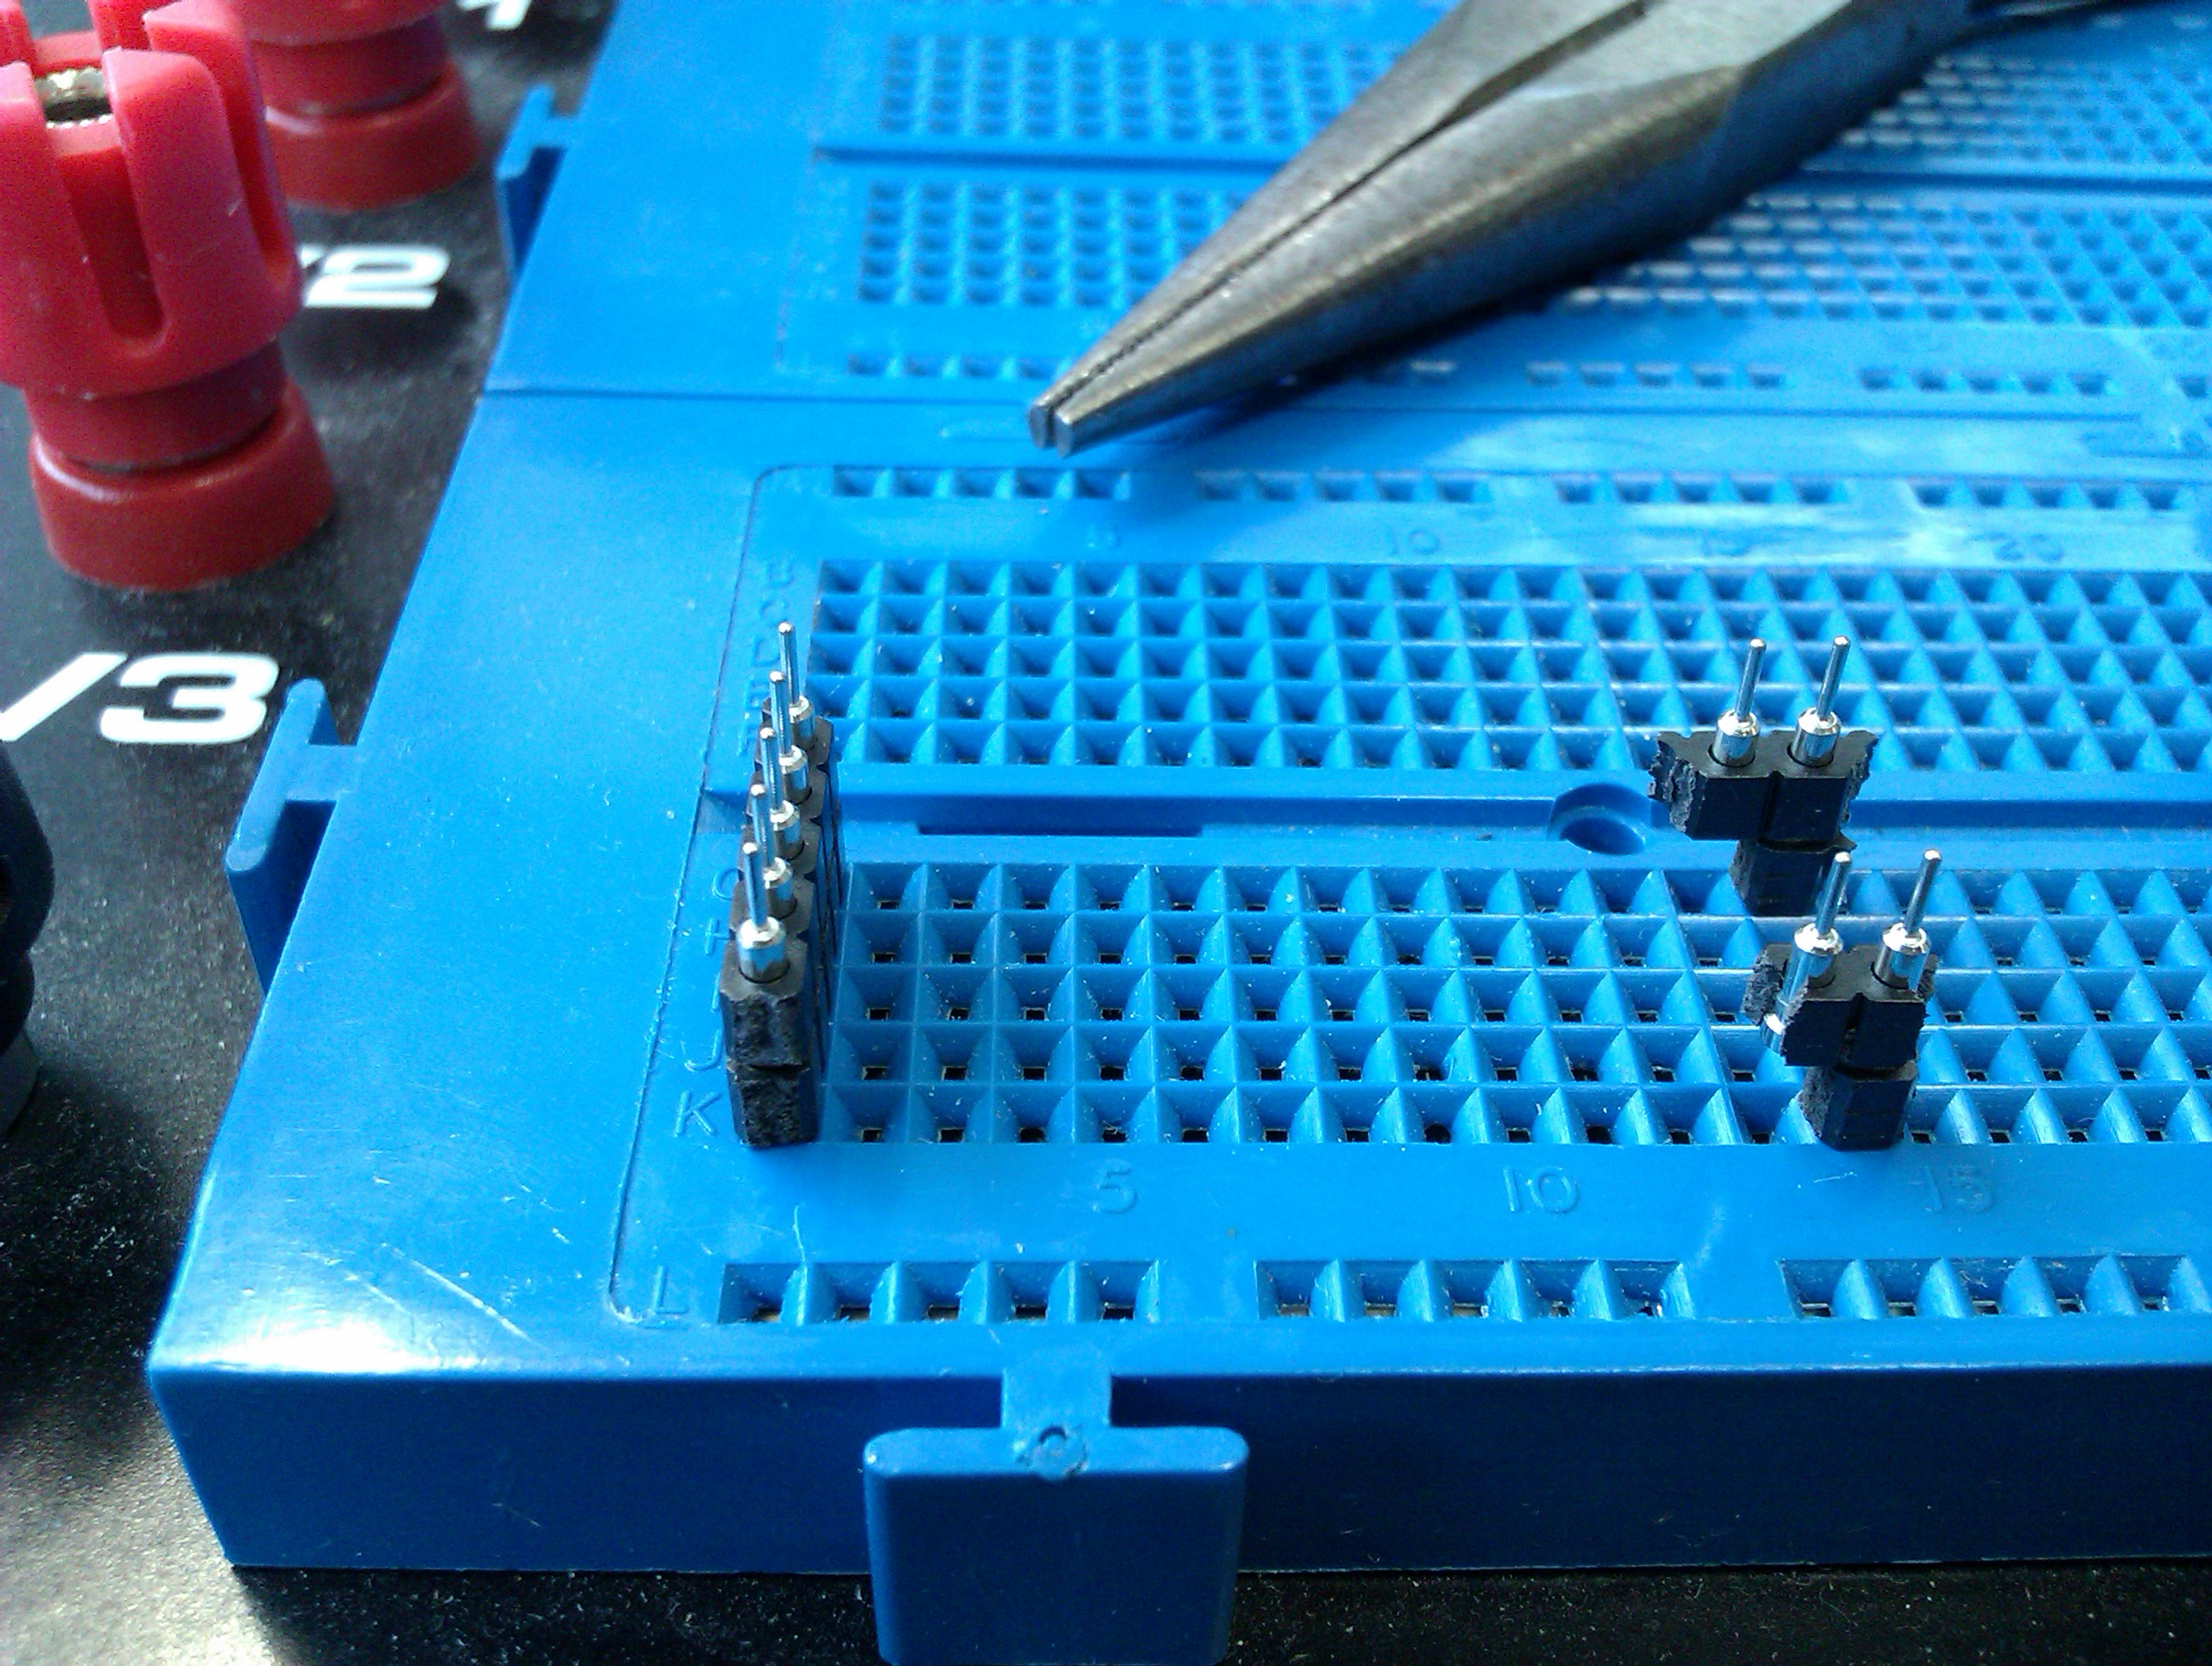
\includegraphics[width=10cm,keepaspectratio]{%
      images/flc100-step-2}
    \caption{Fit the female turned-pin sockets.}
    \label{fig:flc100-step-2}
  \end{figure}
  \begin{figure}[p]
    \centering
    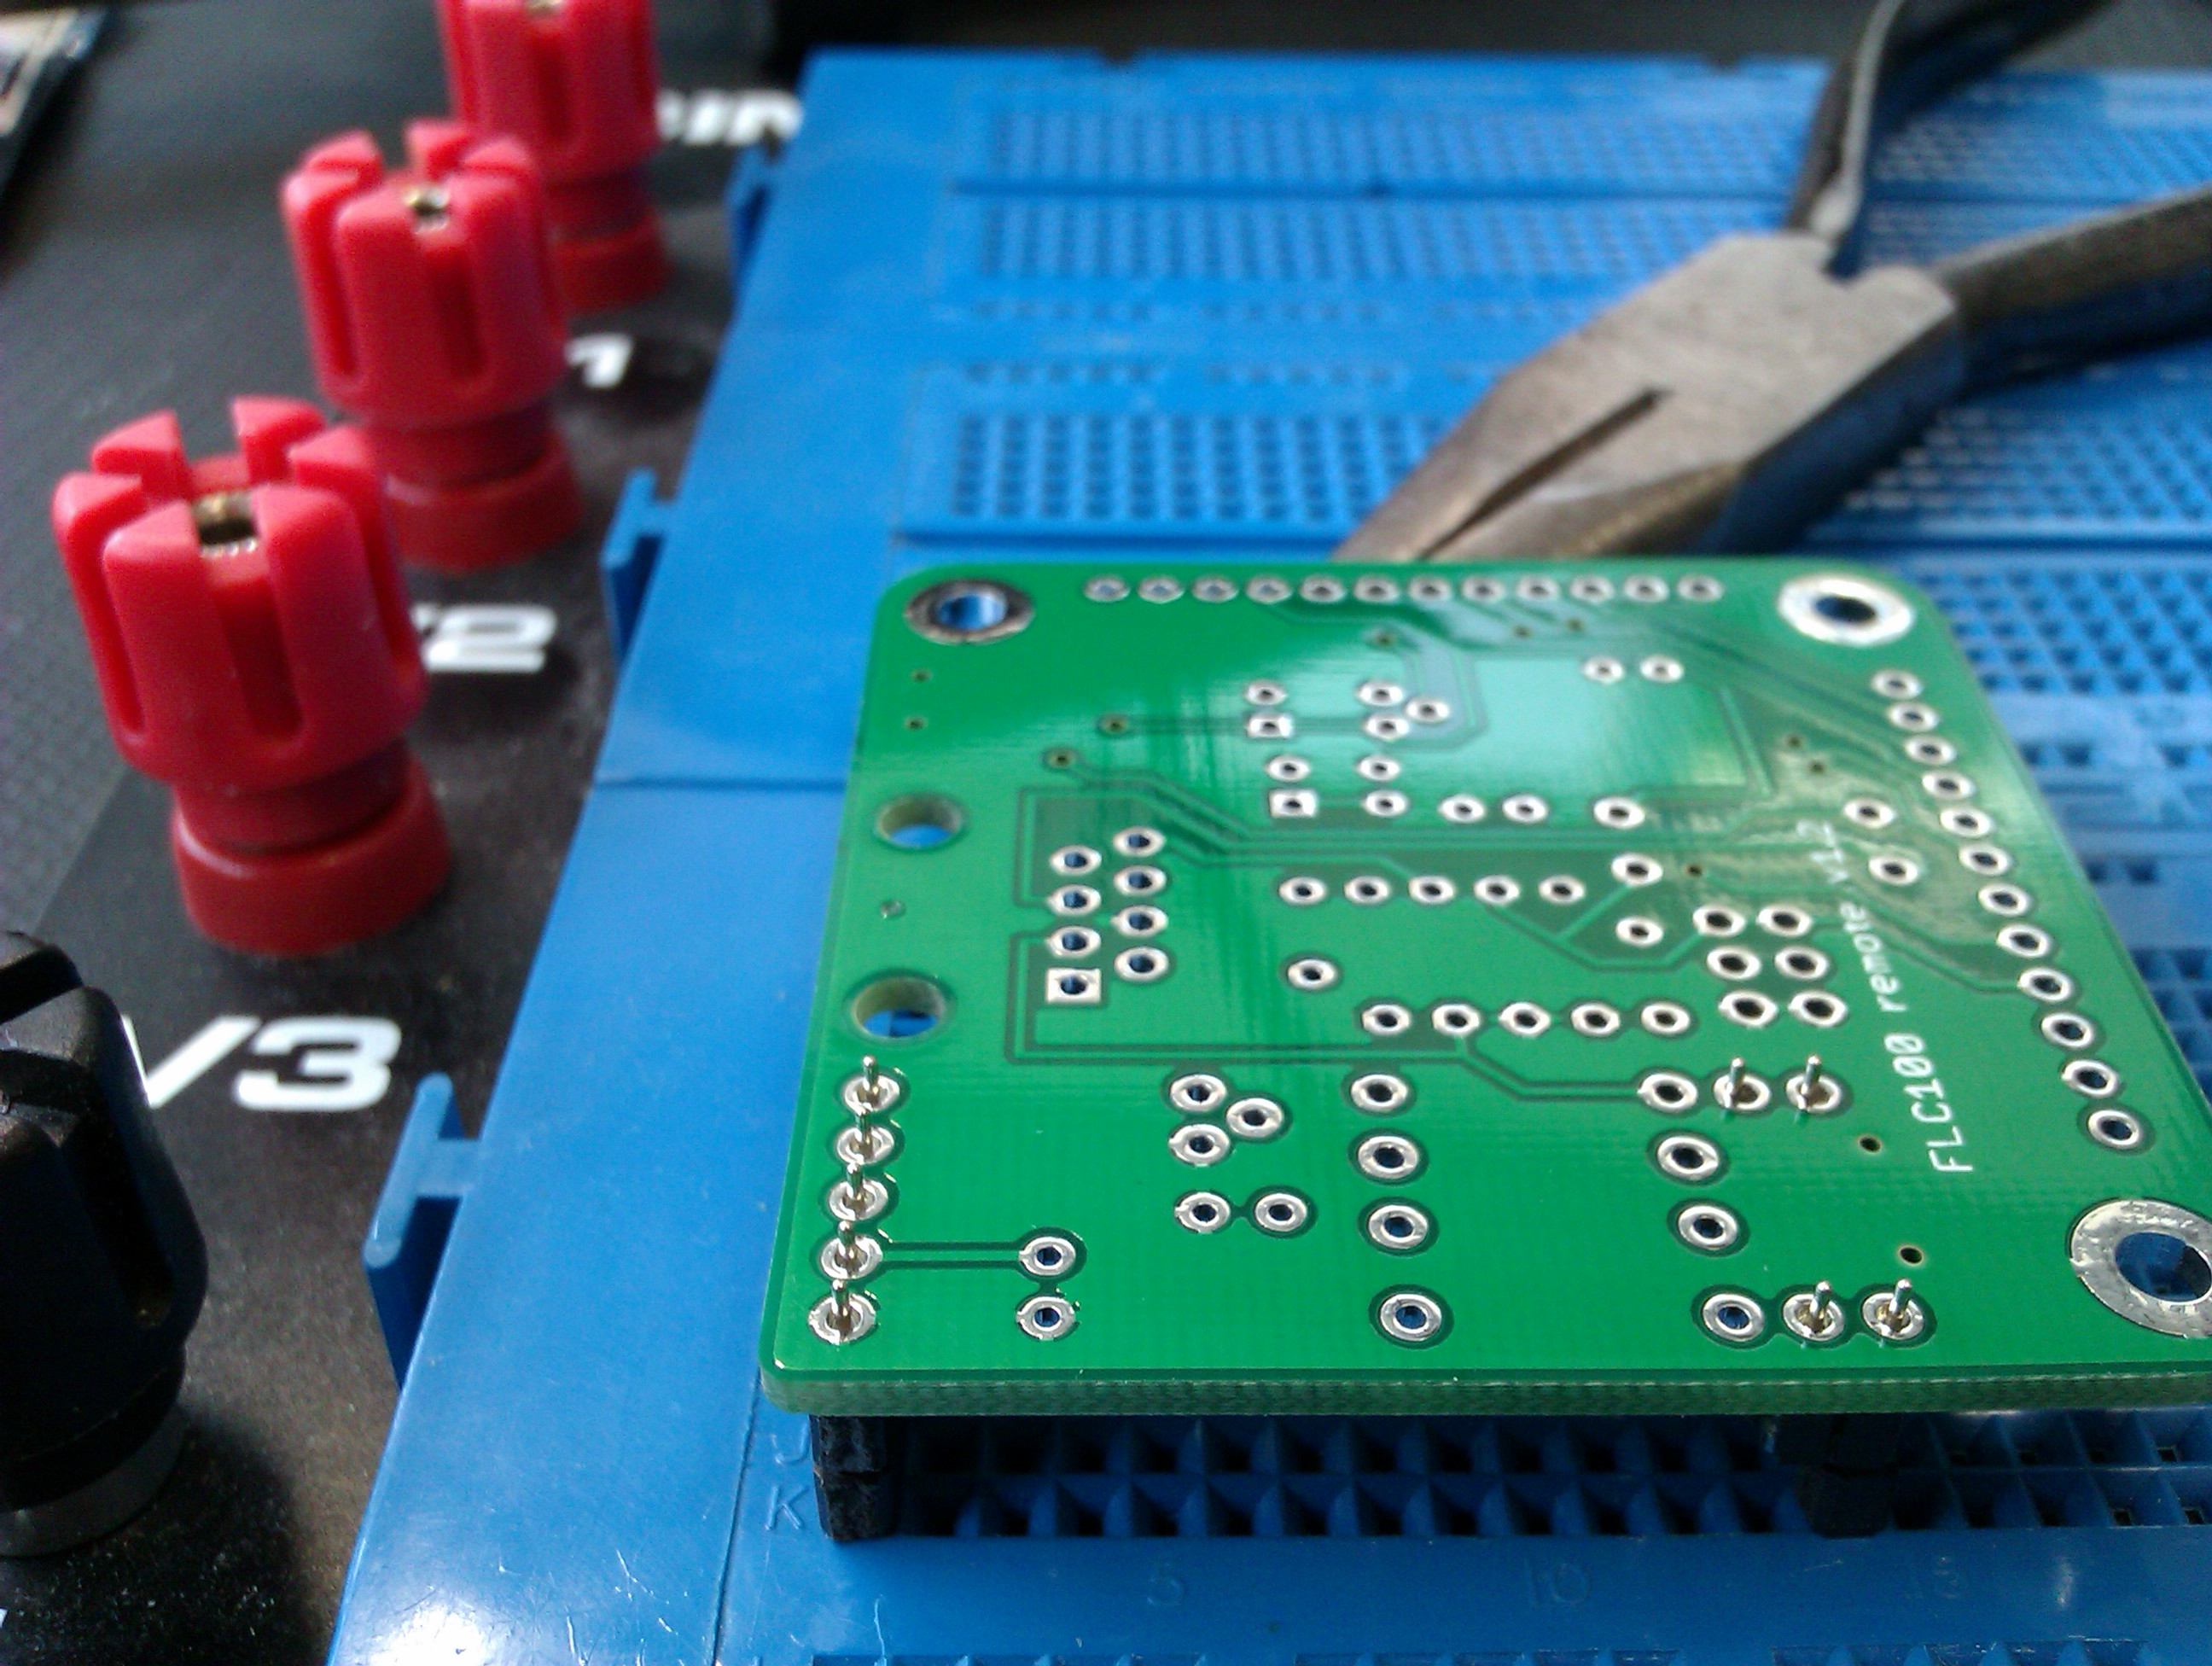
\includegraphics[width=10cm,keepaspectratio]{%
      images/flc100-step-3}
    \caption[Place the sensor PCB onto the female turned-pin
    sockets.]{%
      Place the sensor PCB onto the female turned-pin sockets. The
      pliers are used to support the other side of the PCB.}
    \label{fig:flc100-step-3}
  \end{figure}
\item IC1 (MAXMCP3424).
\item IC2 (MAX619).
\item R1, R2, R3 (\kohm{10}).
\item R4 (\kohm{100}).
\item R5 (\kohm{4.7}).
\item C1, C2, C5, C9 (\nF{100}).
\item C9 (\nF{10}).  
\item C6, C7 (\nF{220}).
\item C3, C4 (\uF{4.7}).
\item D1 (BAT85).
\item SENS2 (LM61).
\item JP5 and JP7 (fit as $2\times3$ male header).
\item X1 (RJ45 vertical jack).
\item Q1 (2N7000). This item is very sensitive to damage by
  electrostatic discharge!
\item SENS1. Gently fit the FLC100 sensor into the turned-pin
  sockets. Apply pressure only on the circuit boards, not the
  components or coil.
\end{buildorder}

\begin{landscape}
  % \thispagestyle{empty}
  \begin{figure}[p]
    \centering
    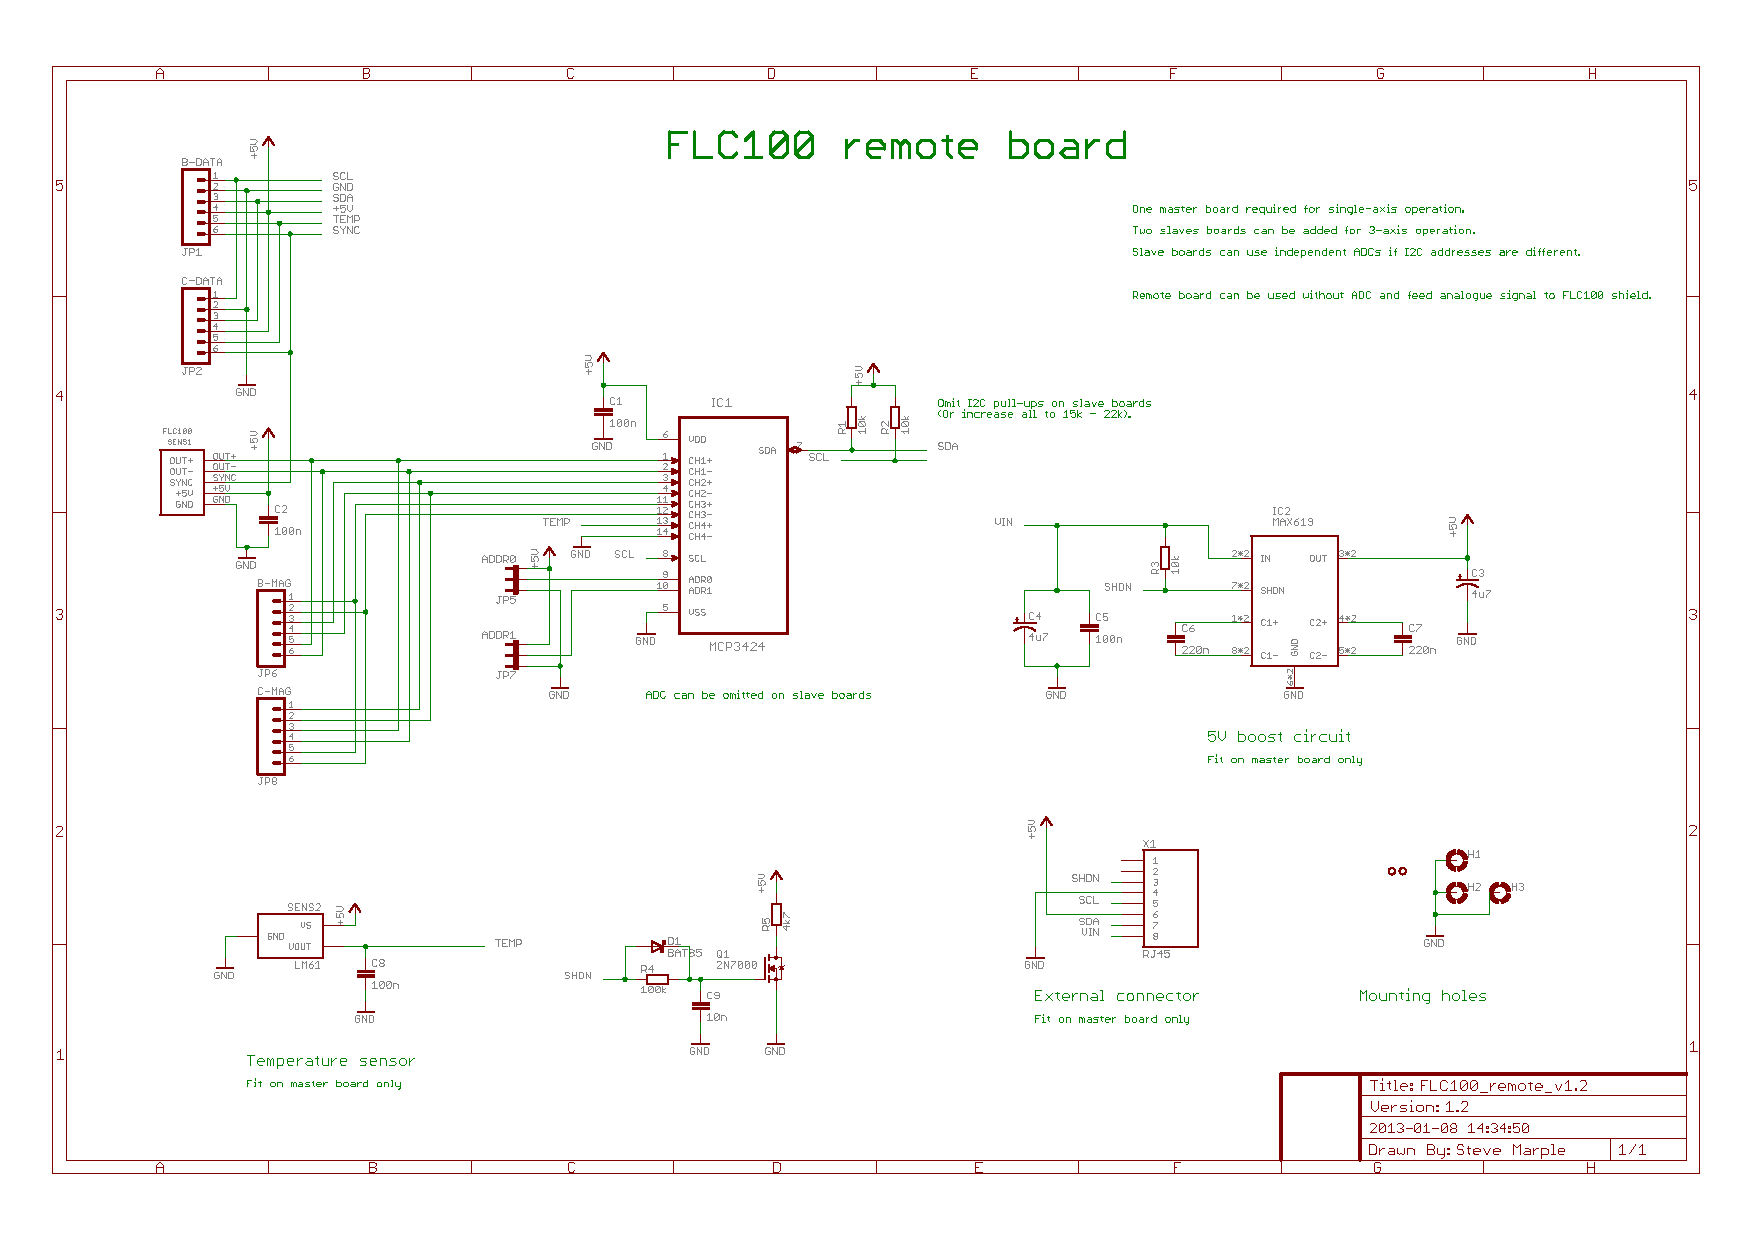
\includegraphics[keepaspectratio,width=28cm,height=16cm]{%
      {../../hardware/FLC100_shield/remote_v1.2/FLC100_remote_v1.2_sch}.pdf}
    \caption{Sensor PCB version 1.2 circuit diagram.}
    \label{fig:sensor-v1.2-pcb-cct-diag}
  \end{figure}
\end{landscape}


\part{Installation}

\chapter{Site requirements}

\section{Sensor requirements}
The site for the sensor should be chosen with regard to the following
requirements (highest priority given first).

\begin{itemize}
\item Within range of the base unit.
\item Away from moving metal objects, for example, trains (more than
  \SI{50}{\metre}), cars (more than \SI{20}{\metre}).
\item Away from static metal objects, in particular those containing
  the \emph{ferro-magnetic} materials iron, nickel and cobalt.
\end{itemize}

\section{Network requirements}

The following network requirements are needed for the system to
operate fully:
\begin{itemize}
\item \dns\ resolution. This is normally provided
  as standard on most networks.
\item Outgoing access on port 123 (\ntp).
\item Outgoing \ssh\ access (port 22).
\end{itemize}






\part{Operation}

\end{document}
